\chapter{Search for CP violation in gluon-gluon fusion events}
\section{Measuring CP violation in gluon-gluon fusion events}%
\subsection{Categorization}%
\subsubsection{0-jet and boosted categories}%
\begin{figure}[h!]
    \centering
    \begin{subfigure}{.3\textwidth}
        \centering
        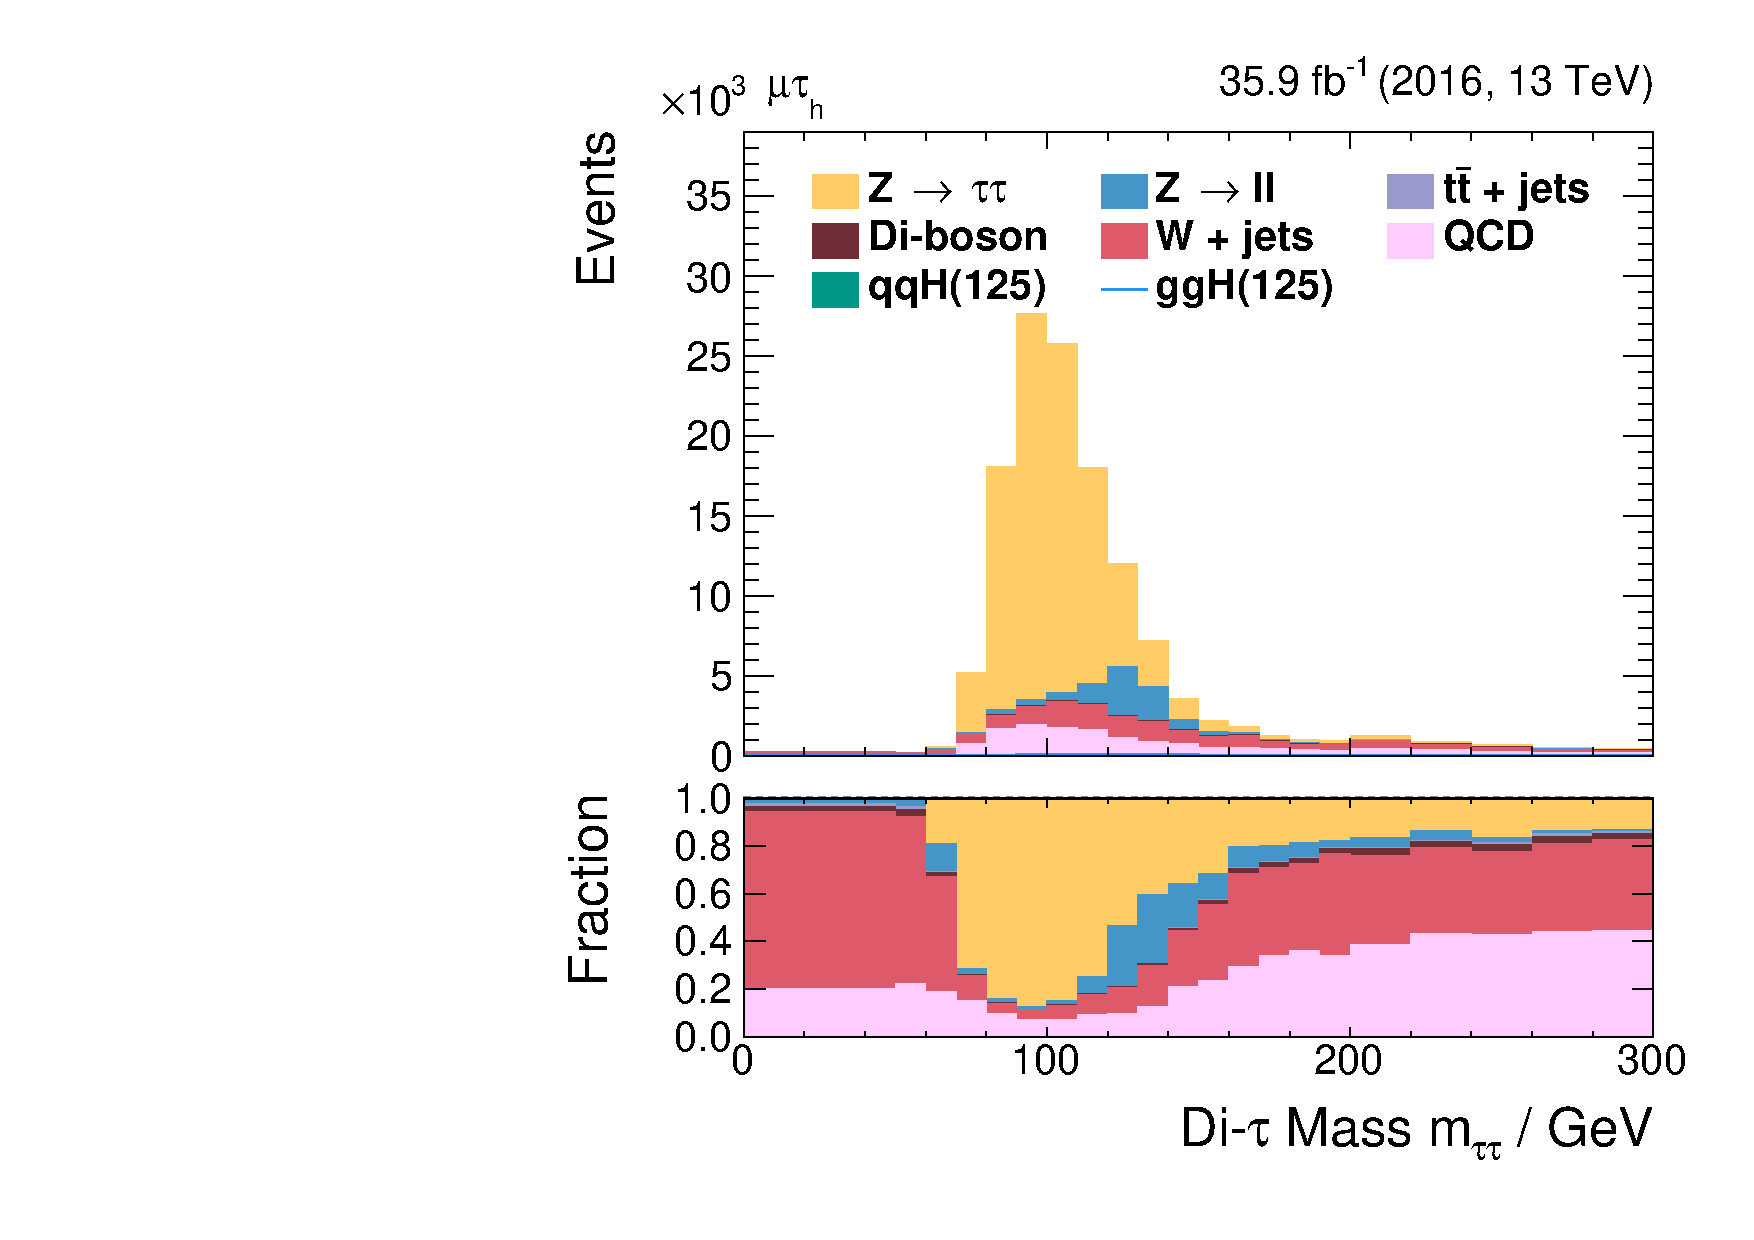
\includegraphics[width=\textwidth]{Figures/eventselection/mt/ZeroJetCP/m_sv.pdf}
    \end{subfigure}%
    \begin{subfigure}{.3\textwidth}
        \centering
        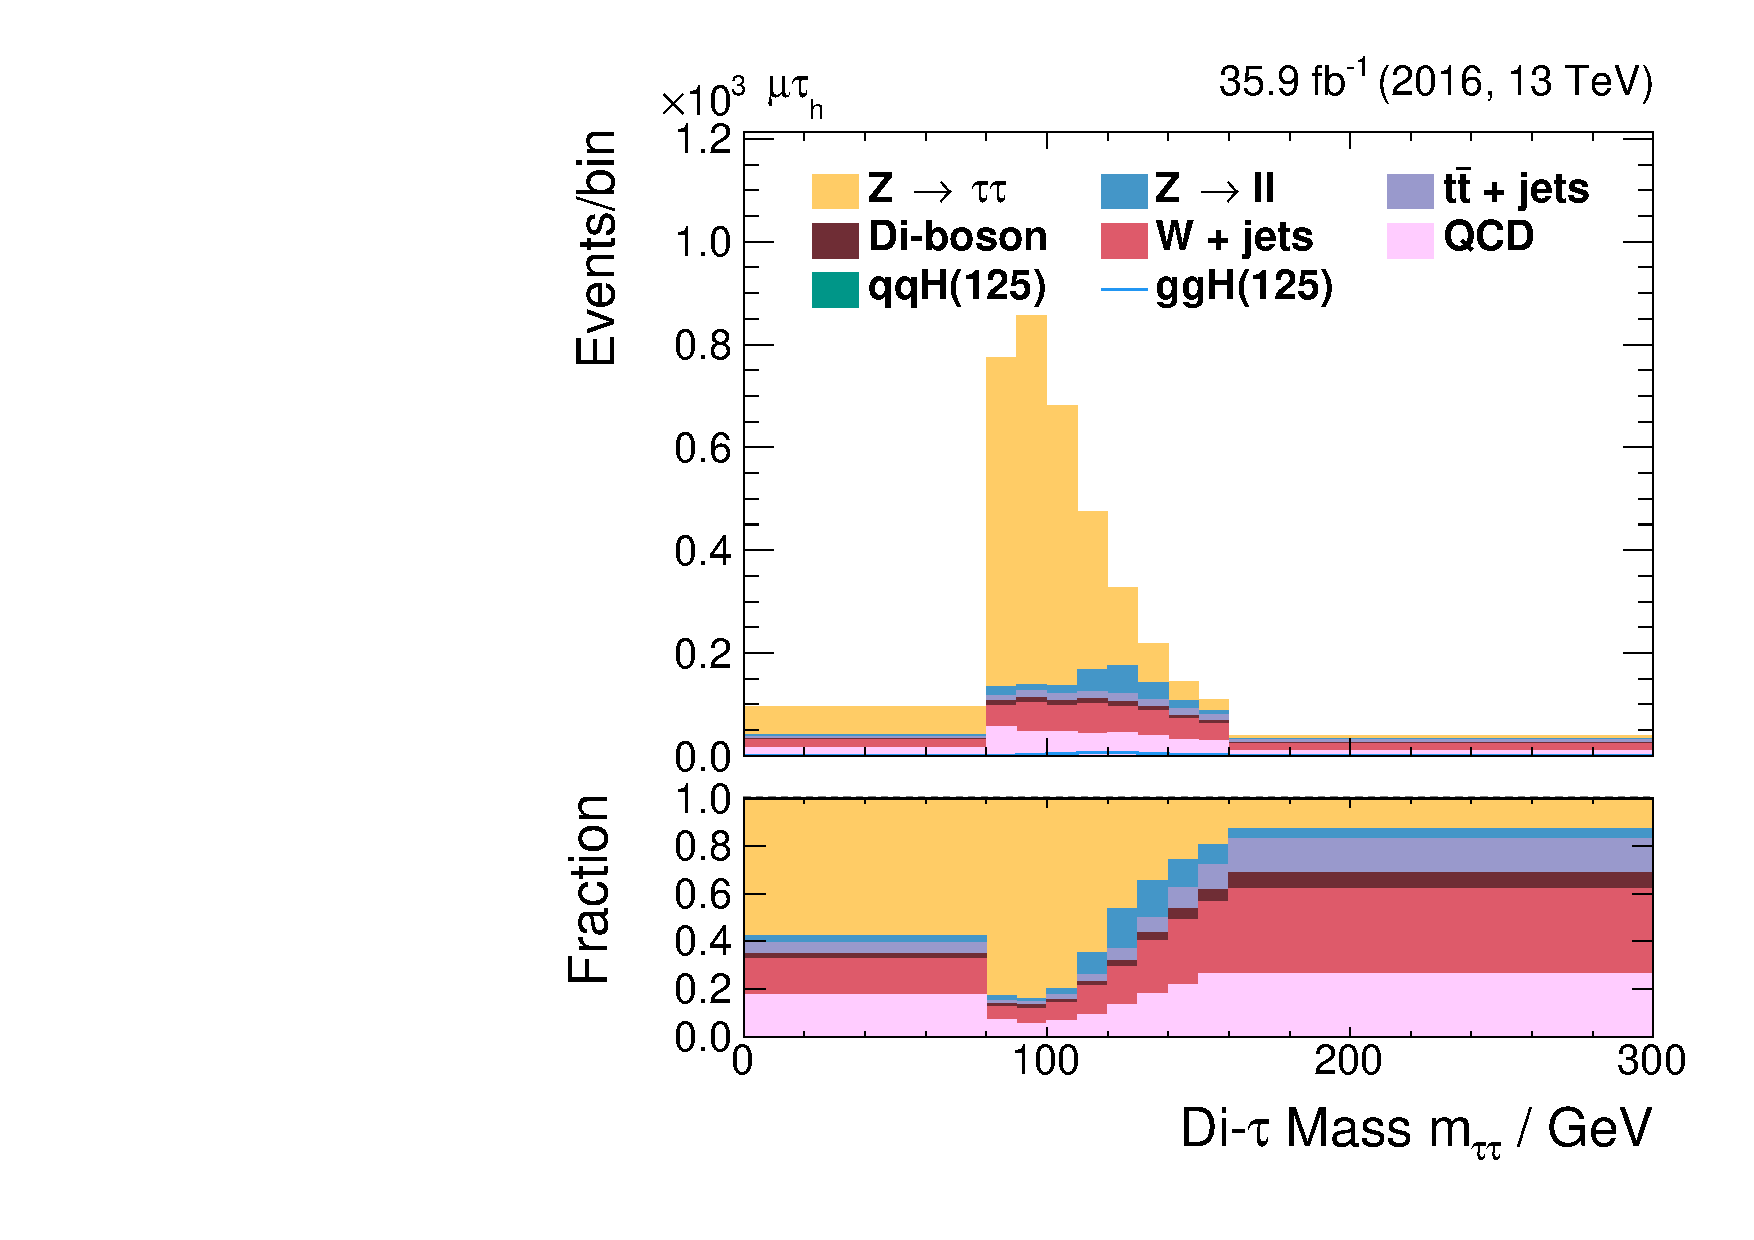
\includegraphics[width=\textwidth]{Figures/eventselection/mt/BoostedCP/m_sv.pdf}
    \end{subfigure}%
    \begin{subfigure}{.3\textwidth}
        \centering
        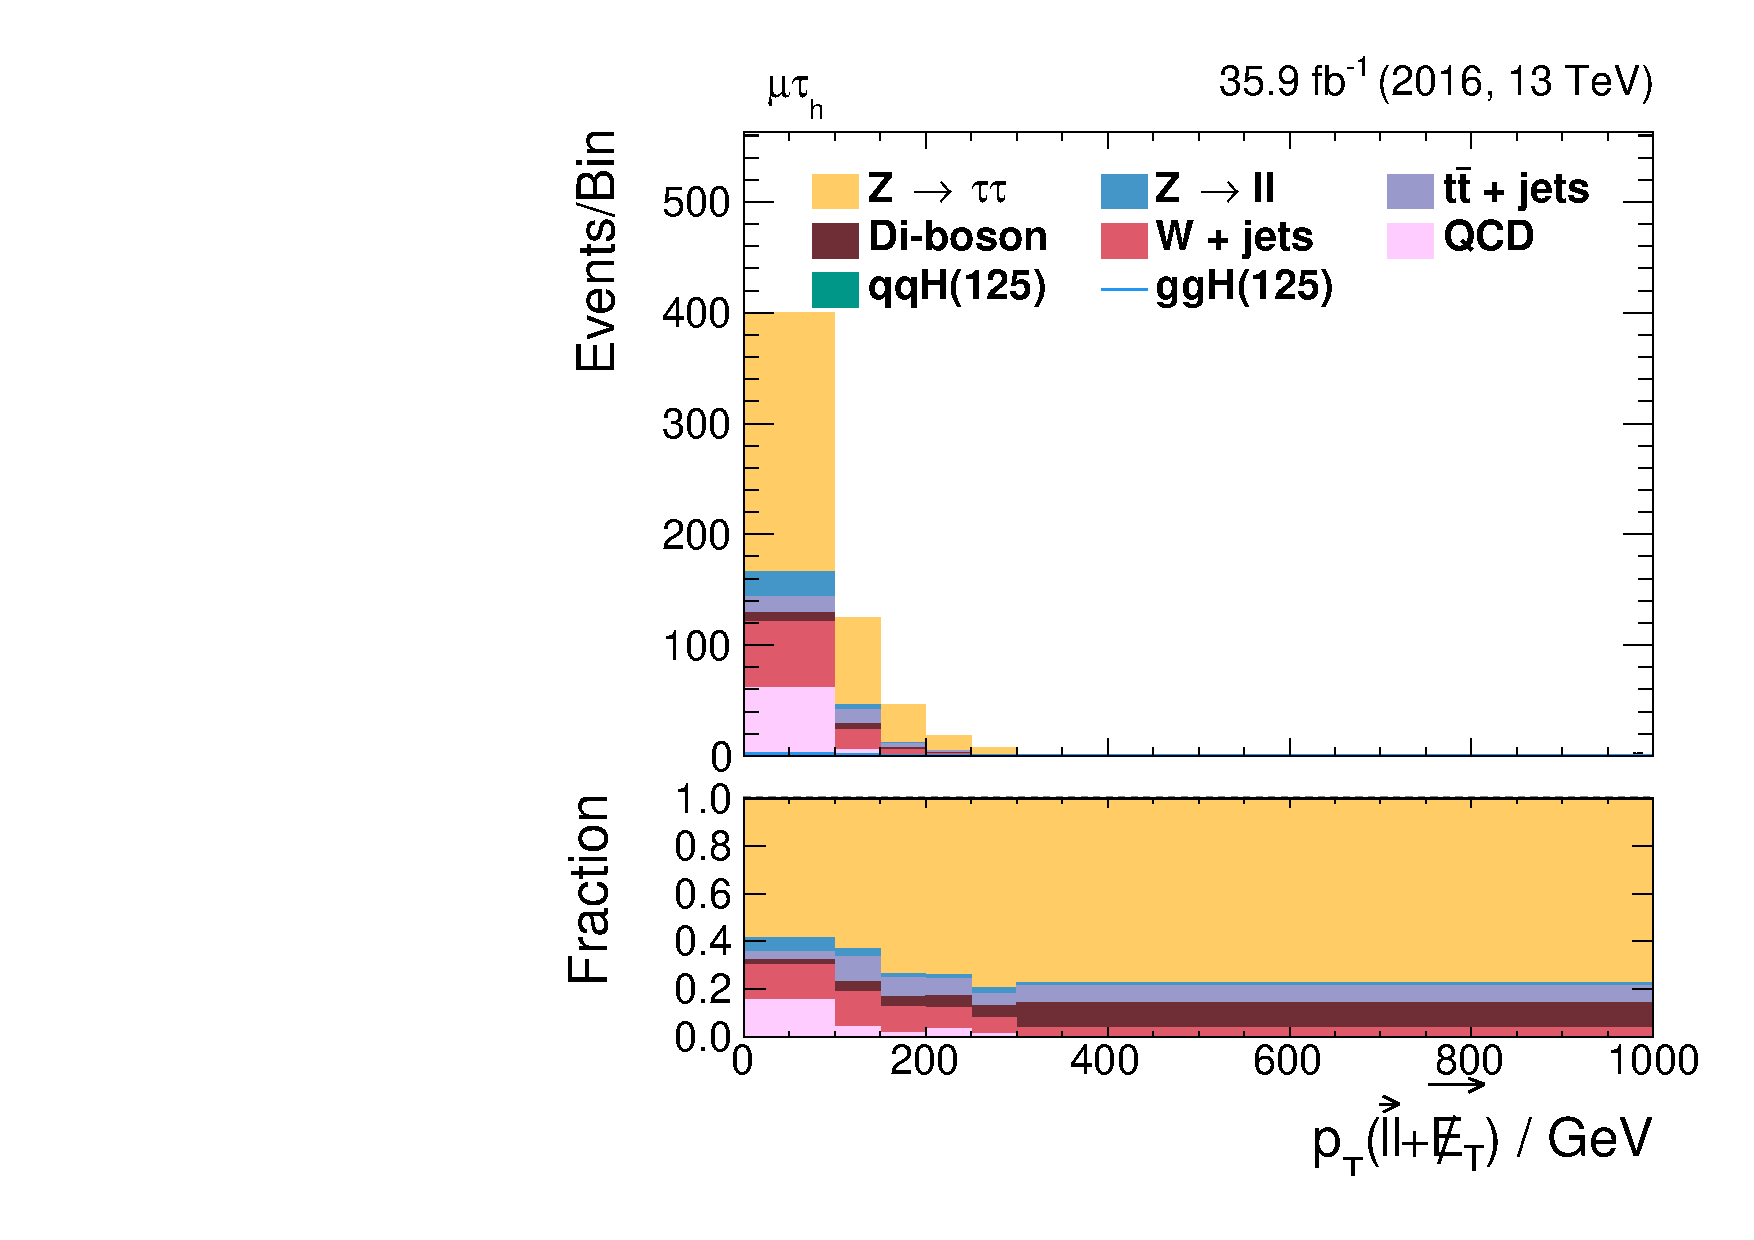
\includegraphics[width=\textwidth]{Figures/eventselection/mt/BoostedCP/H_pt.pdf}
    \end{subfigure} \\ %
    \begin{subfigure}{.3\textwidth}
        \centering
        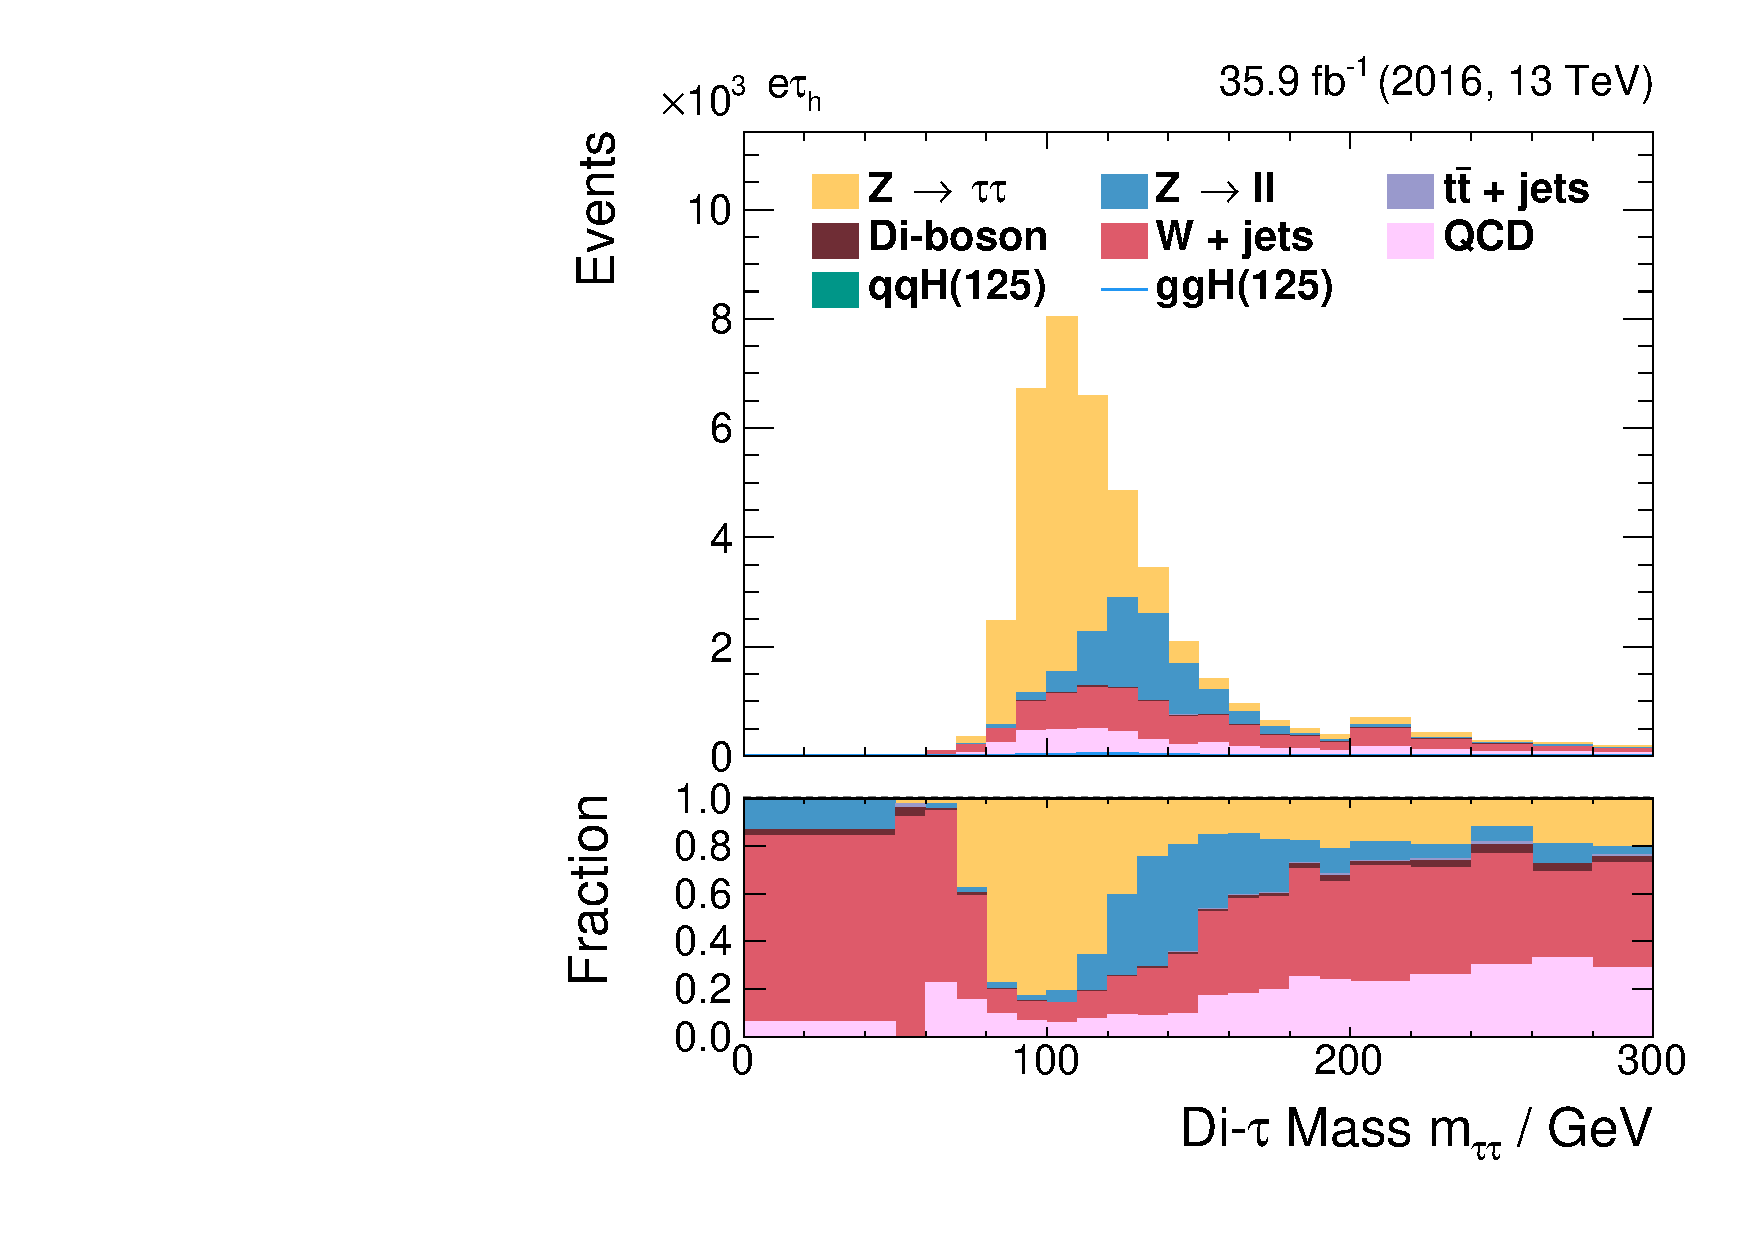
\includegraphics[width=\textwidth]{Figures/eventselection/et/ZeroJetCP/m_sv.pdf}
    \end{subfigure}%
    \begin{subfigure}{.3\textwidth}
        \centering
        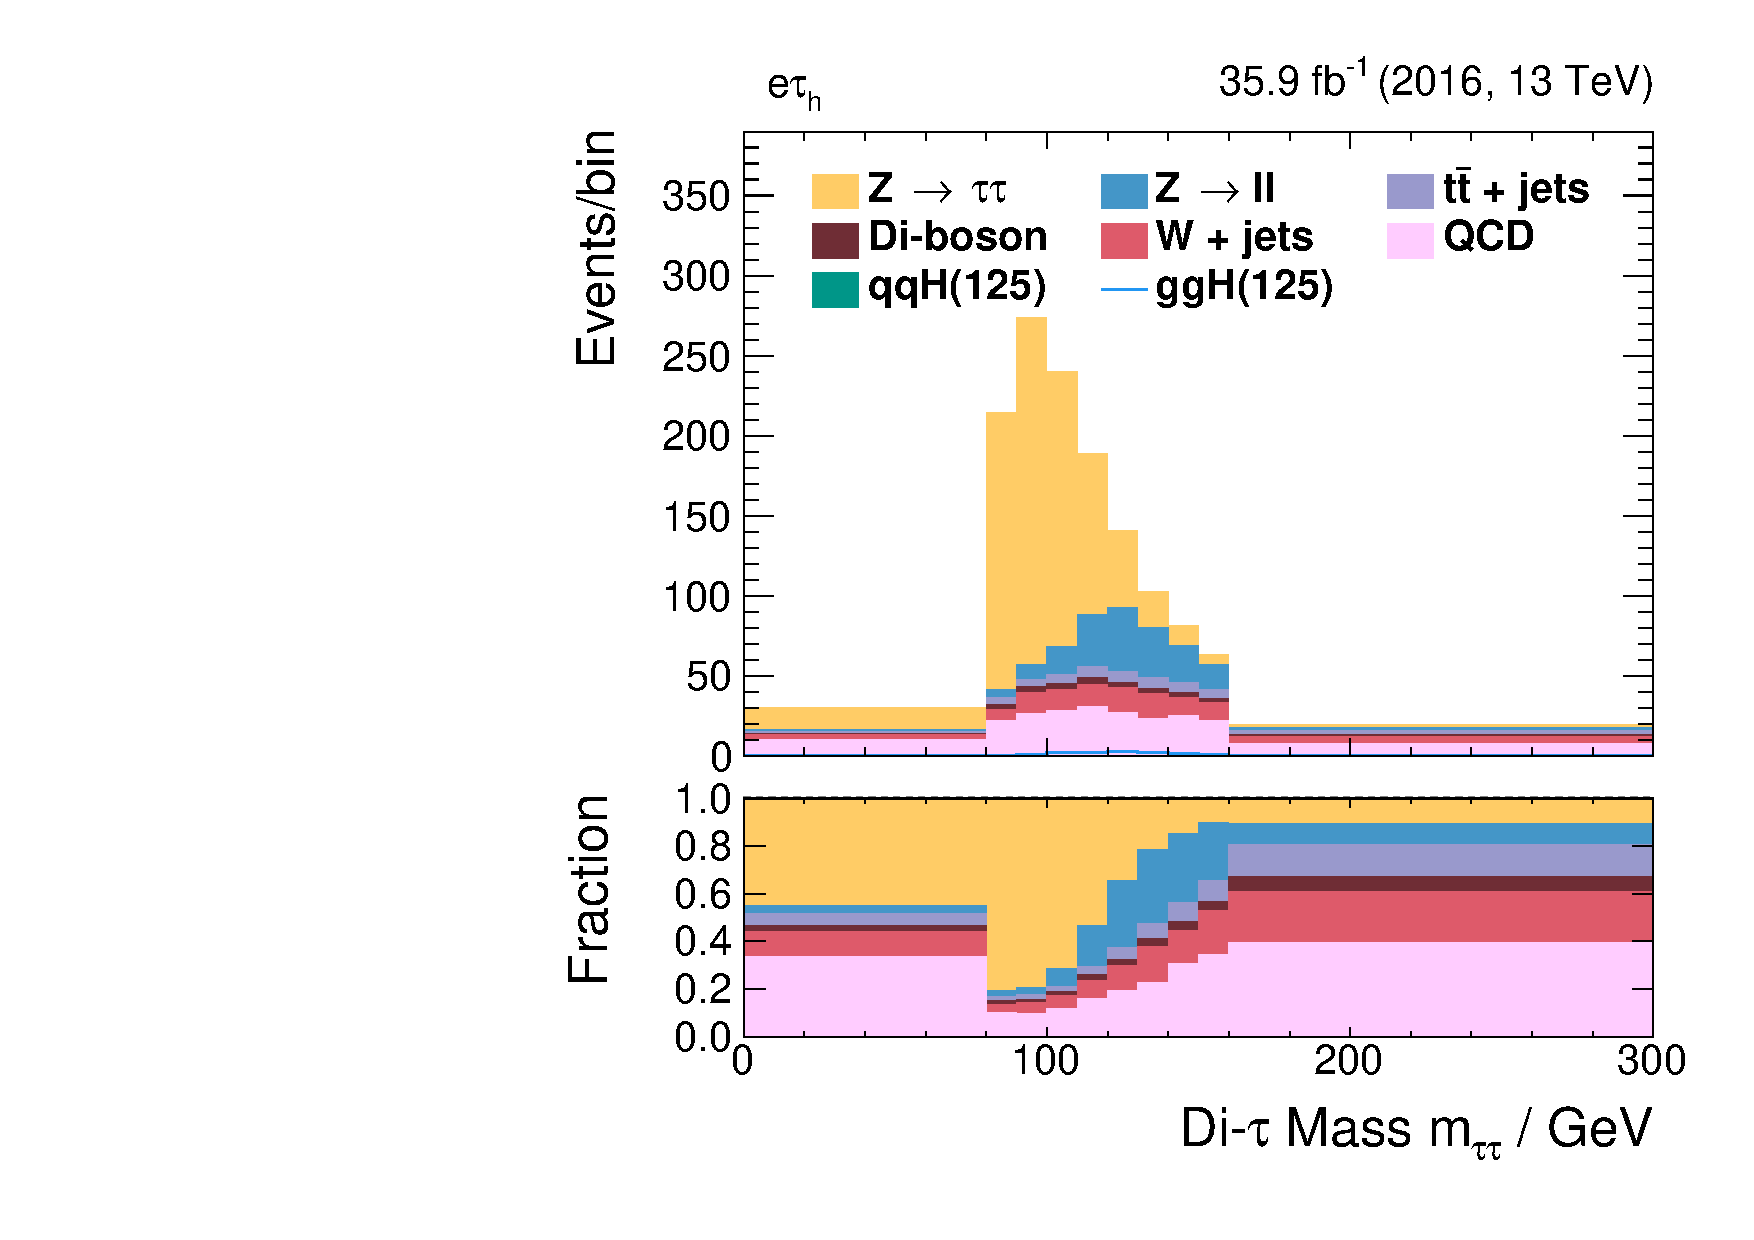
\includegraphics[width=\textwidth]{Figures/eventselection/et/BoostedCP/m_sv.pdf}
    \end{subfigure}%
    \begin{subfigure}{.3\textwidth}
        \centering
        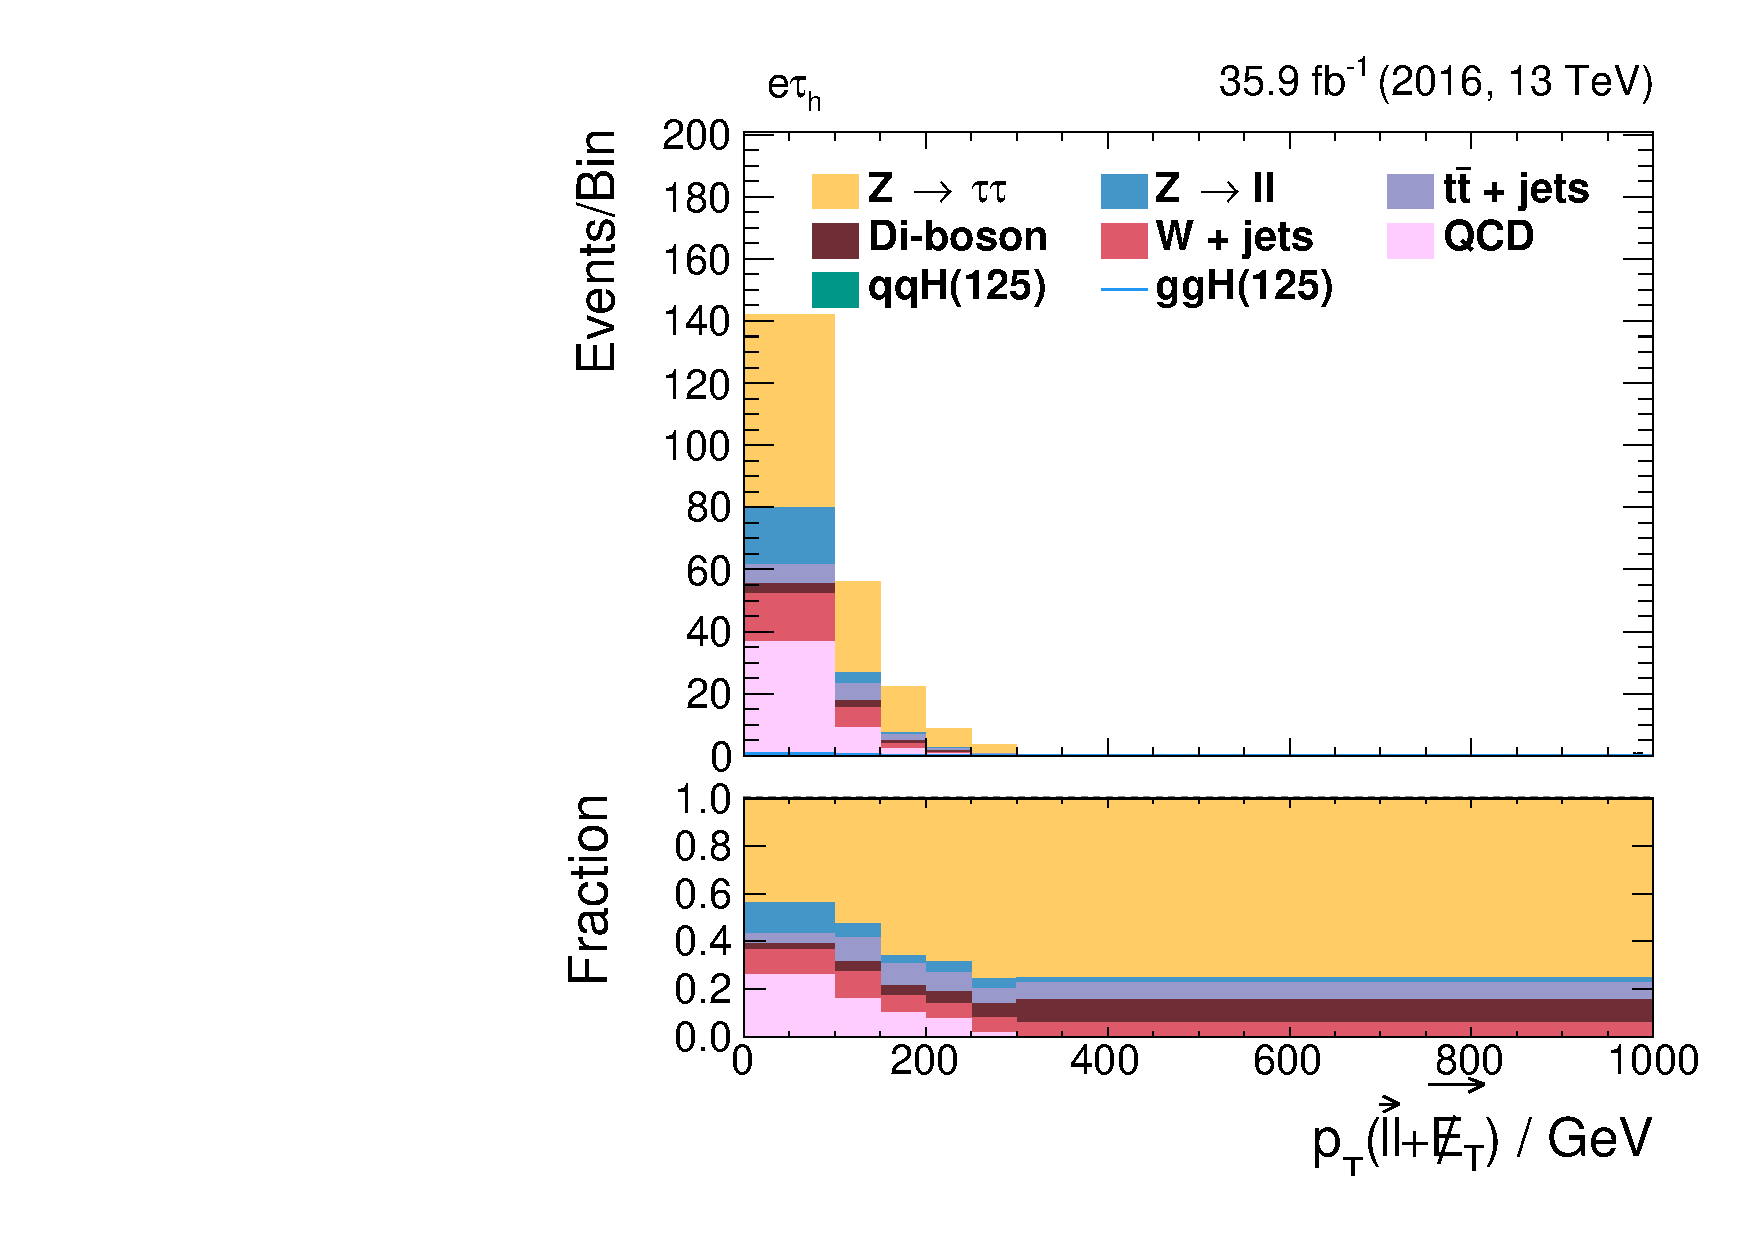
\includegraphics[width=\textwidth]{Figures/eventselection/et/BoostedCP/H_pt.pdf}
    \end{subfigure} \\
    \begin{subfigure}{.3\textwidth}
        \centering
        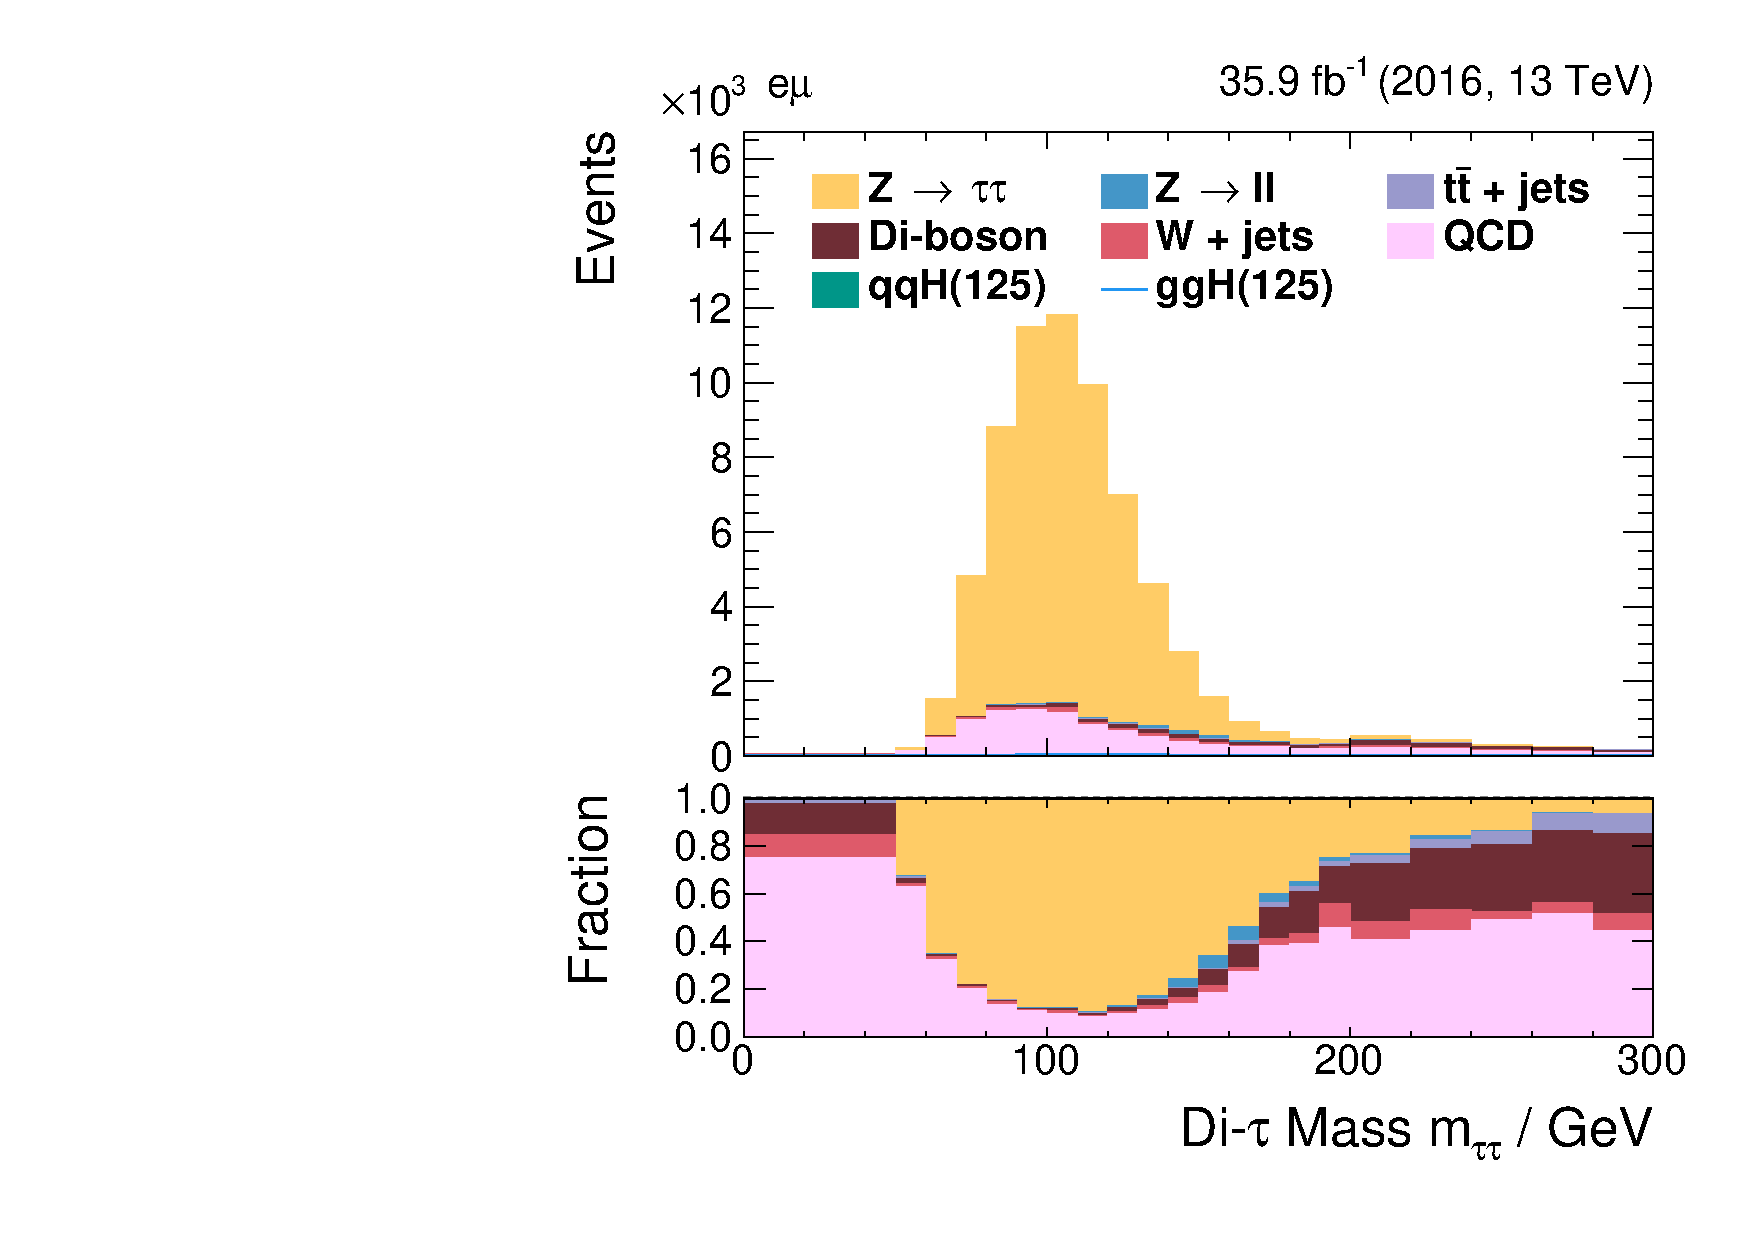
\includegraphics[width=\textwidth]{Figures/eventselection/em/ZeroJetCP/m_sv.pdf}
    \end{subfigure}%
    \begin{subfigure}{.3\textwidth}
        \centering
        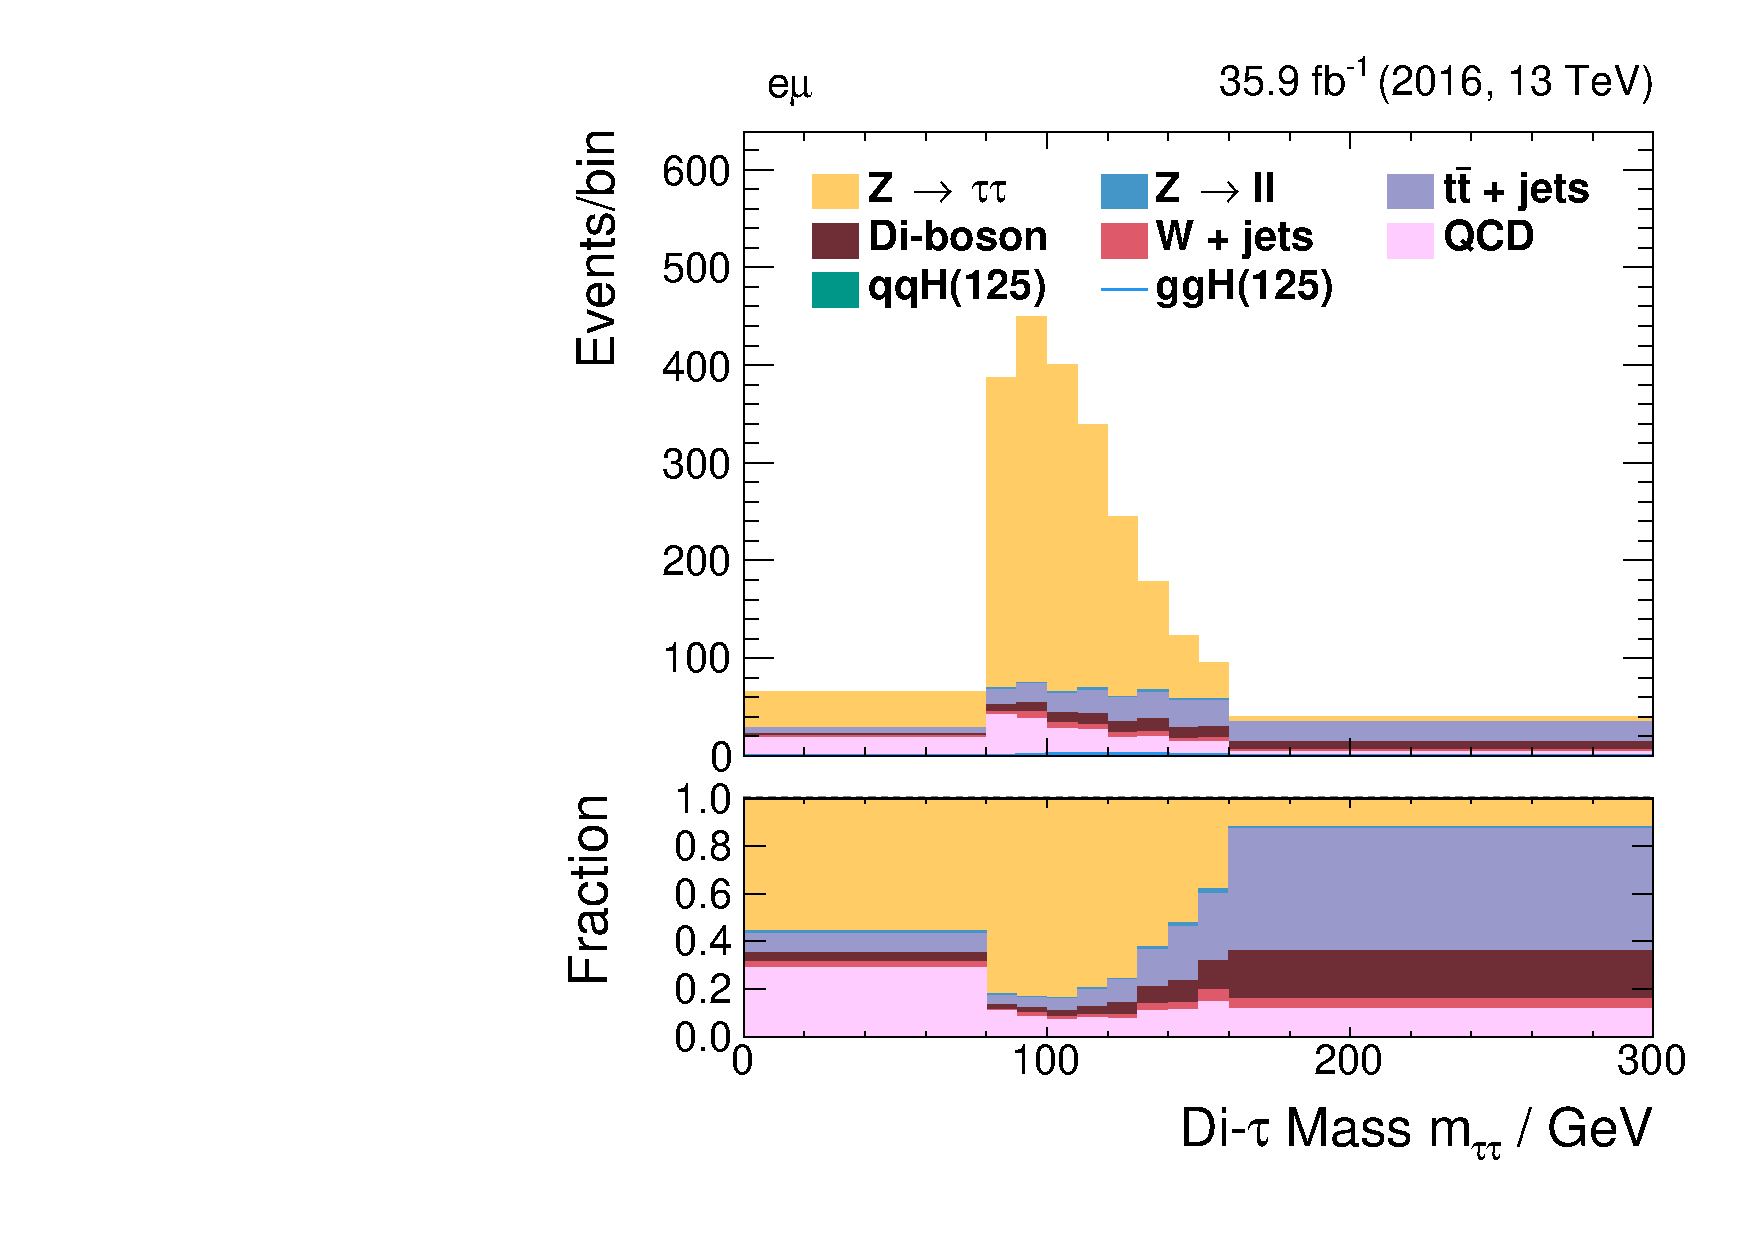
\includegraphics[width=\textwidth]{Figures/eventselection/em/BoostedCP/m_sv.pdf}
    \end{subfigure}%
    \begin{subfigure}{.3\textwidth}
        \centering
        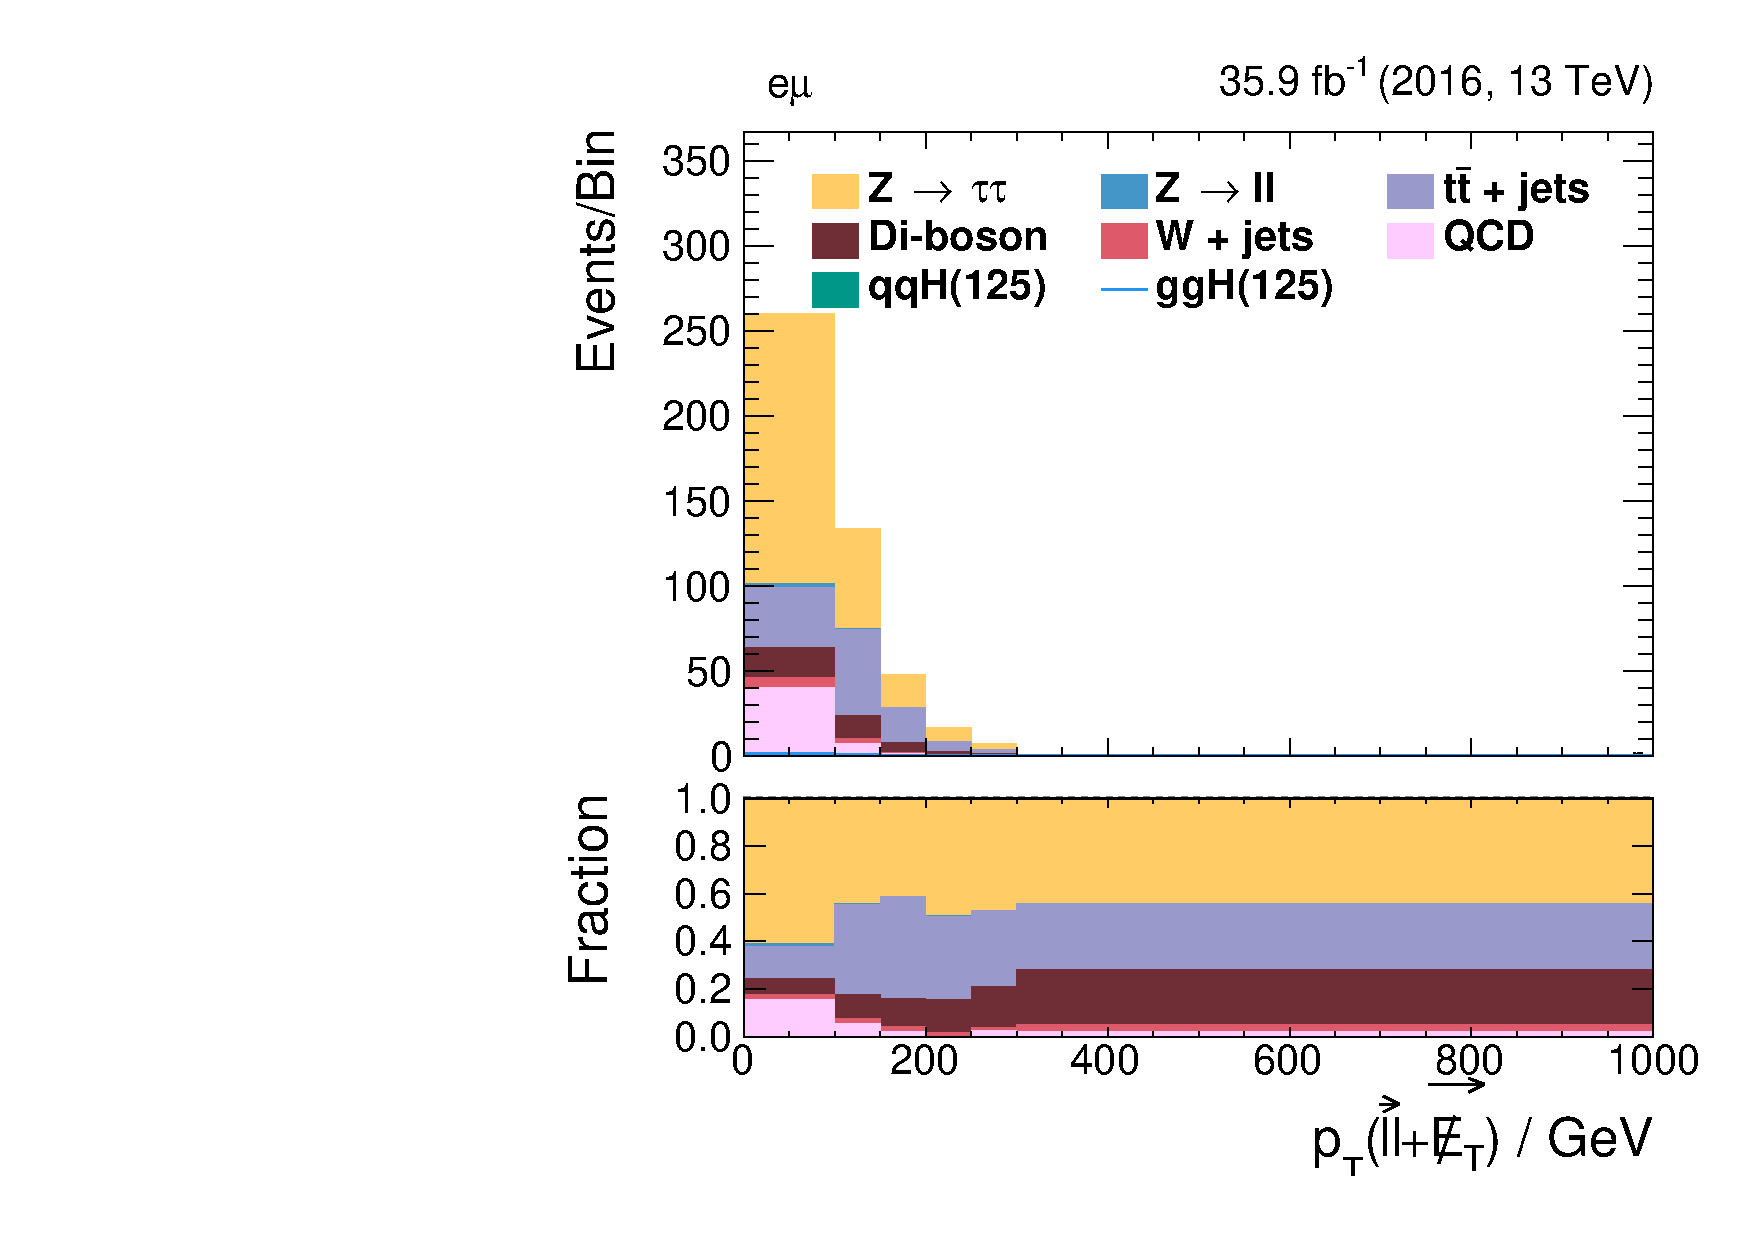
\includegraphics[width=\textwidth]{Figures/eventselection/em/BoostedCP/H_pt.pdf}
    \end{subfigure}
    \caption{Background and expected qqH and ggH signal distributions of observables in the 0-jet category (left) and \textit{boosted} category (middle,right) for the \mutau{} (upper row), \etau{} (middle row) and $e\mu$ (bottom row) channels. 
    The subplot shows the relative fraction of each background in each bin. }\label{SUPPLEMENT:ES:controlplots:0jet_boosted}  
\end{figure}%
\clearpage
\subsubsection{Dijet signal categories}%

\begin{figure}[h!]
    \centering
    \begin{subfigure}{.45\textwidth}
        \centering
        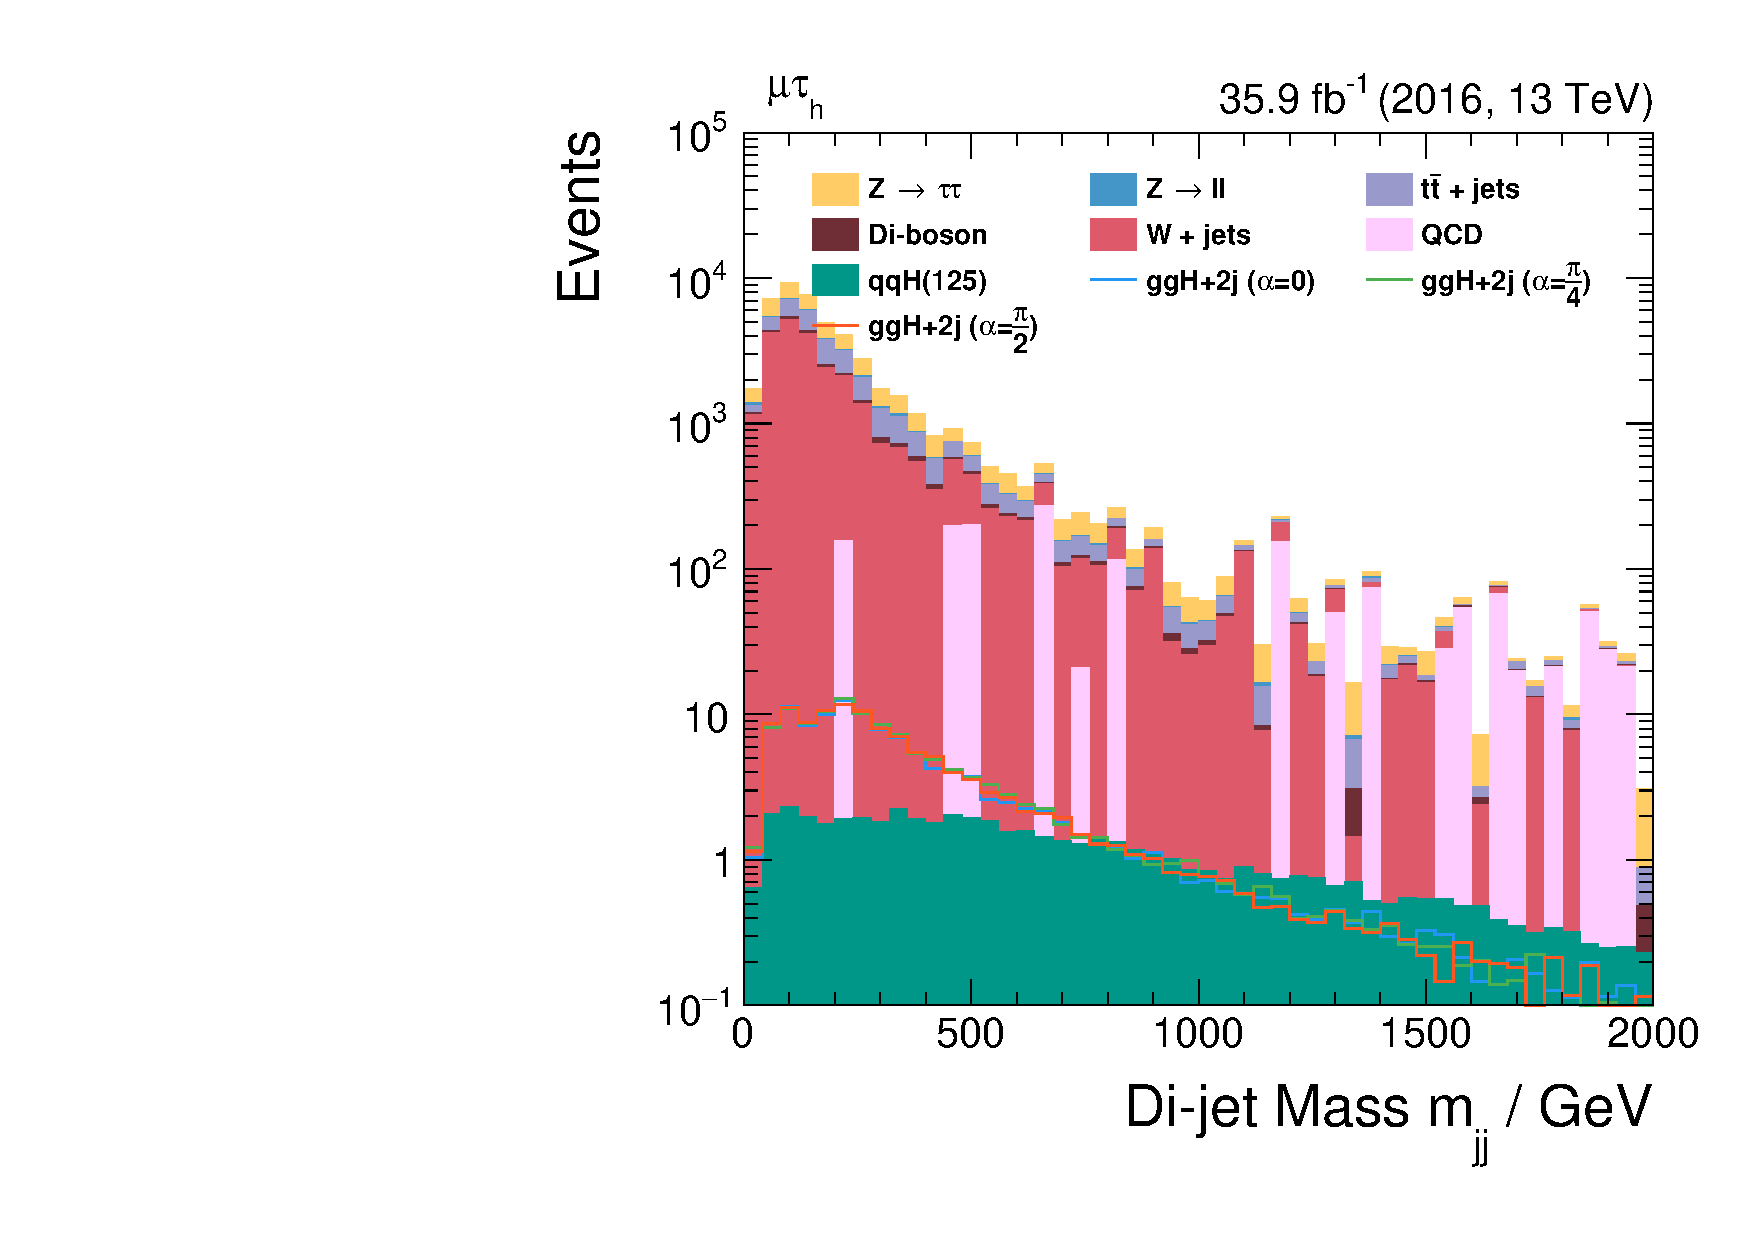
\includegraphics[width=\textwidth]{Figures/eventselection/Categorization/mt/mjj.pdf}
    \end{subfigure}%
    \begin{subfigure}{.45\textwidth}
        \centering
        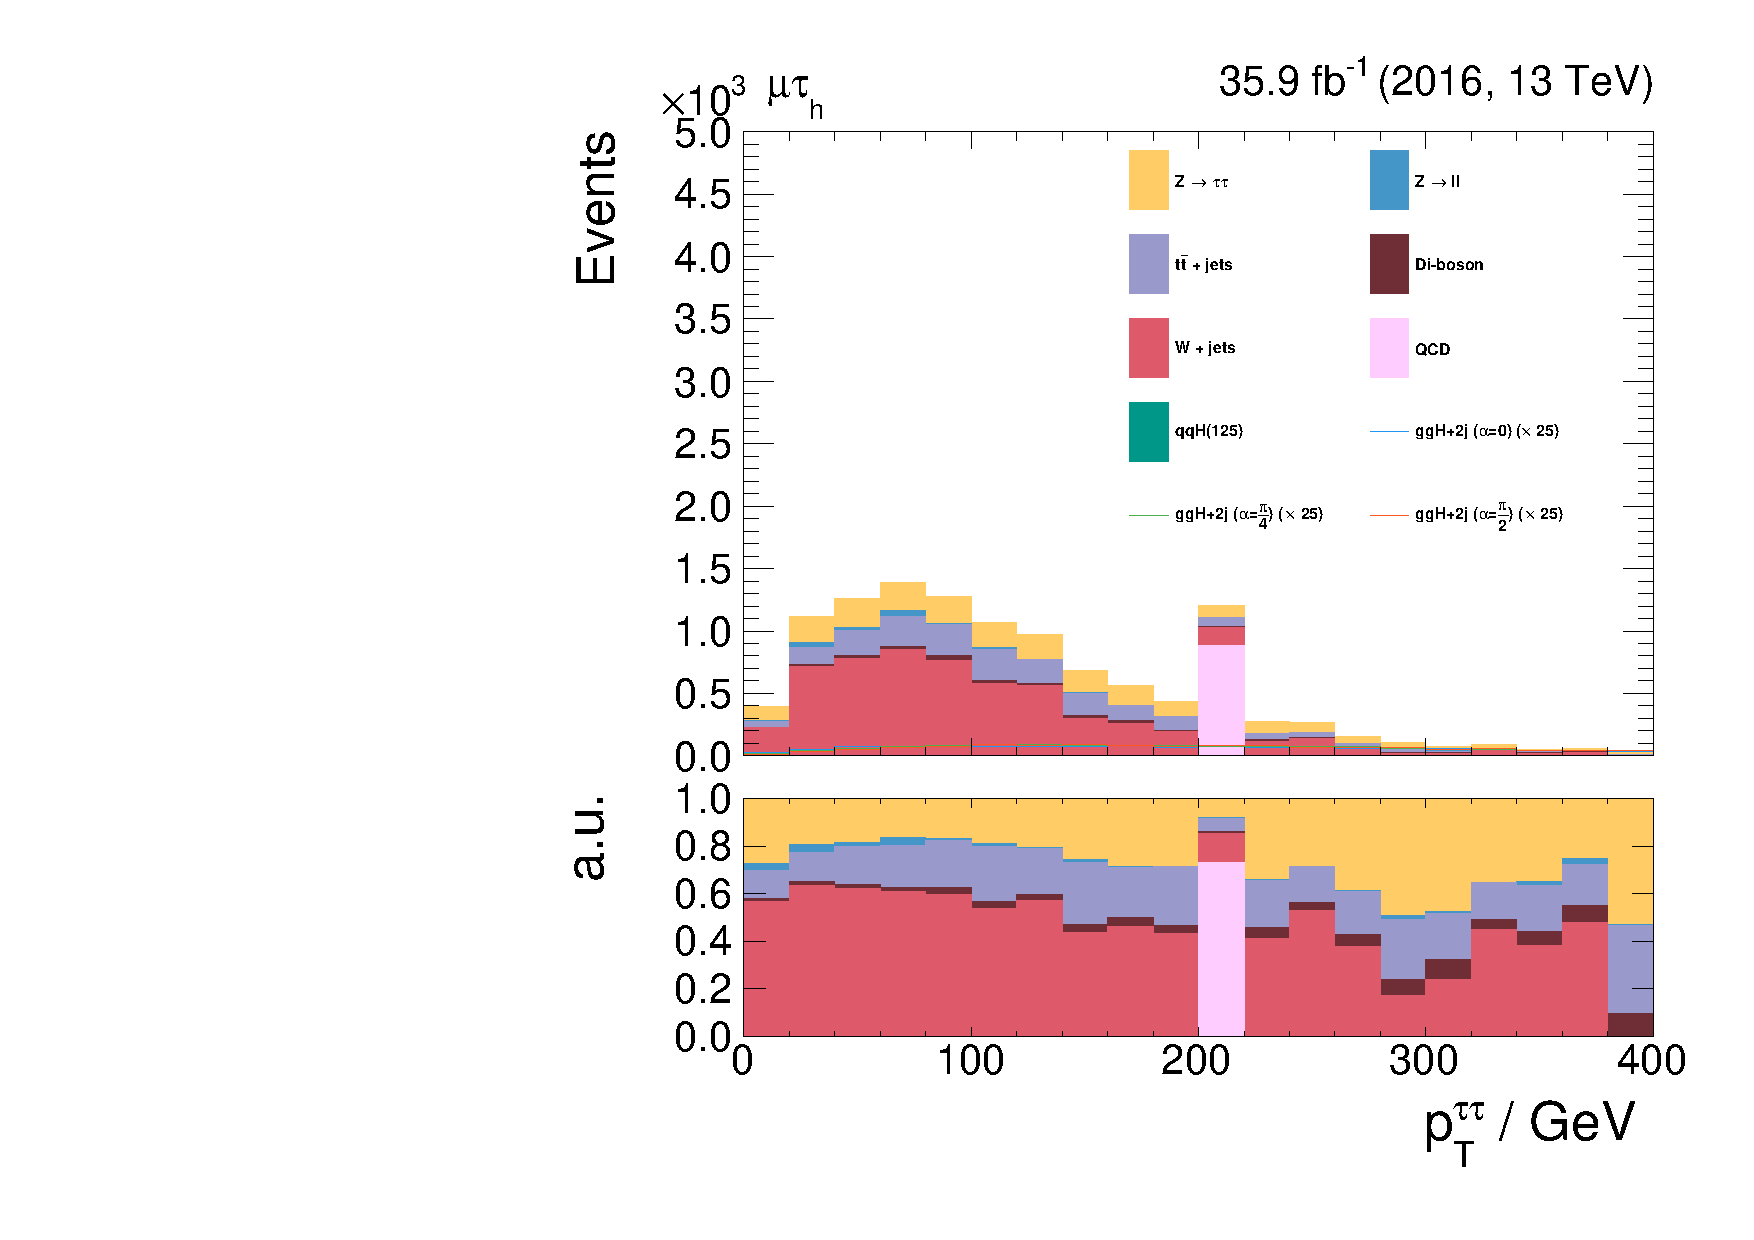
\includegraphics[width=\textwidth]{Figures/eventselection/Categorization/mt/H_pt.pdf}
    \end{subfigure} \\ % 
    \begin{subfigure}{.45\textwidth}
        \centering
        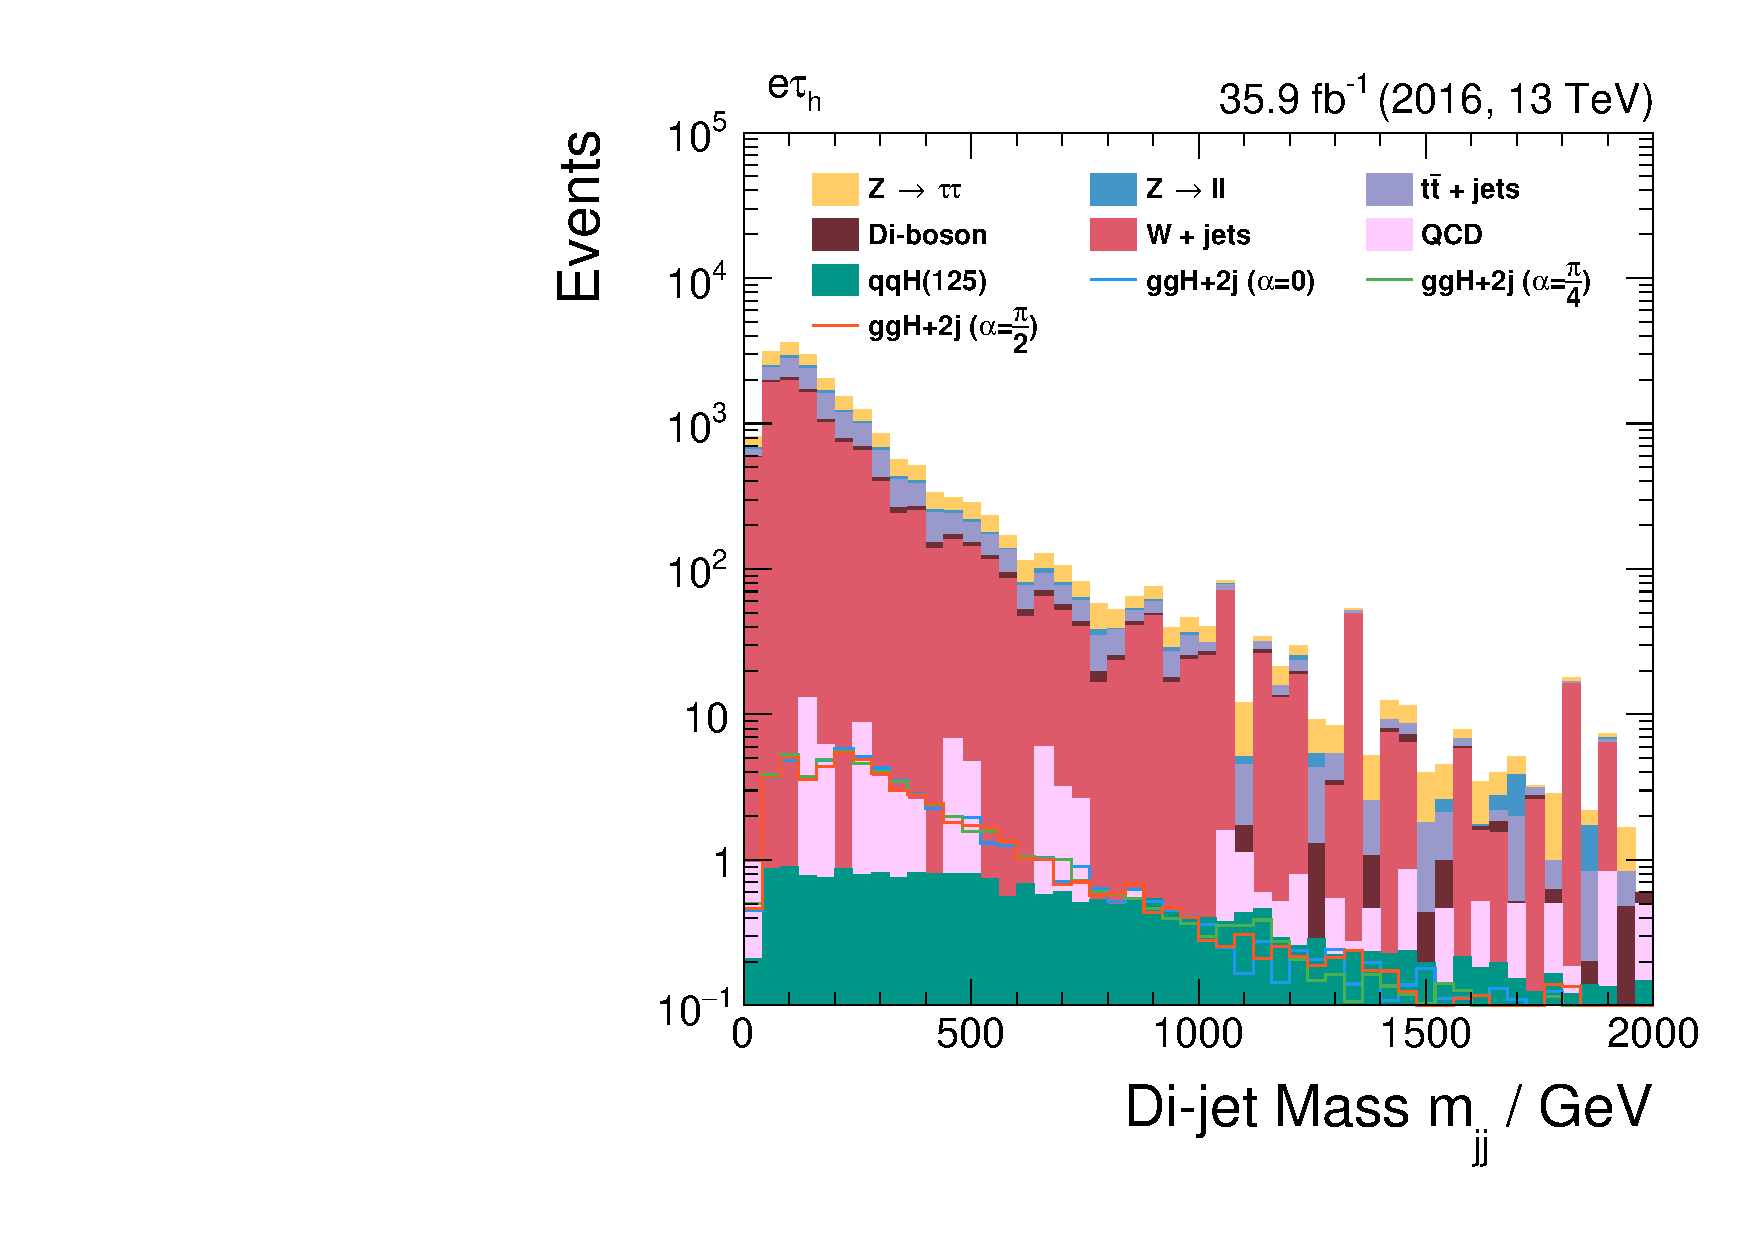
\includegraphics[width=\textwidth]{Figures/eventselection/Categorization/et/mjj.pdf}
    \end{subfigure}%
    \begin{subfigure}{.45\textwidth}
        \centering
        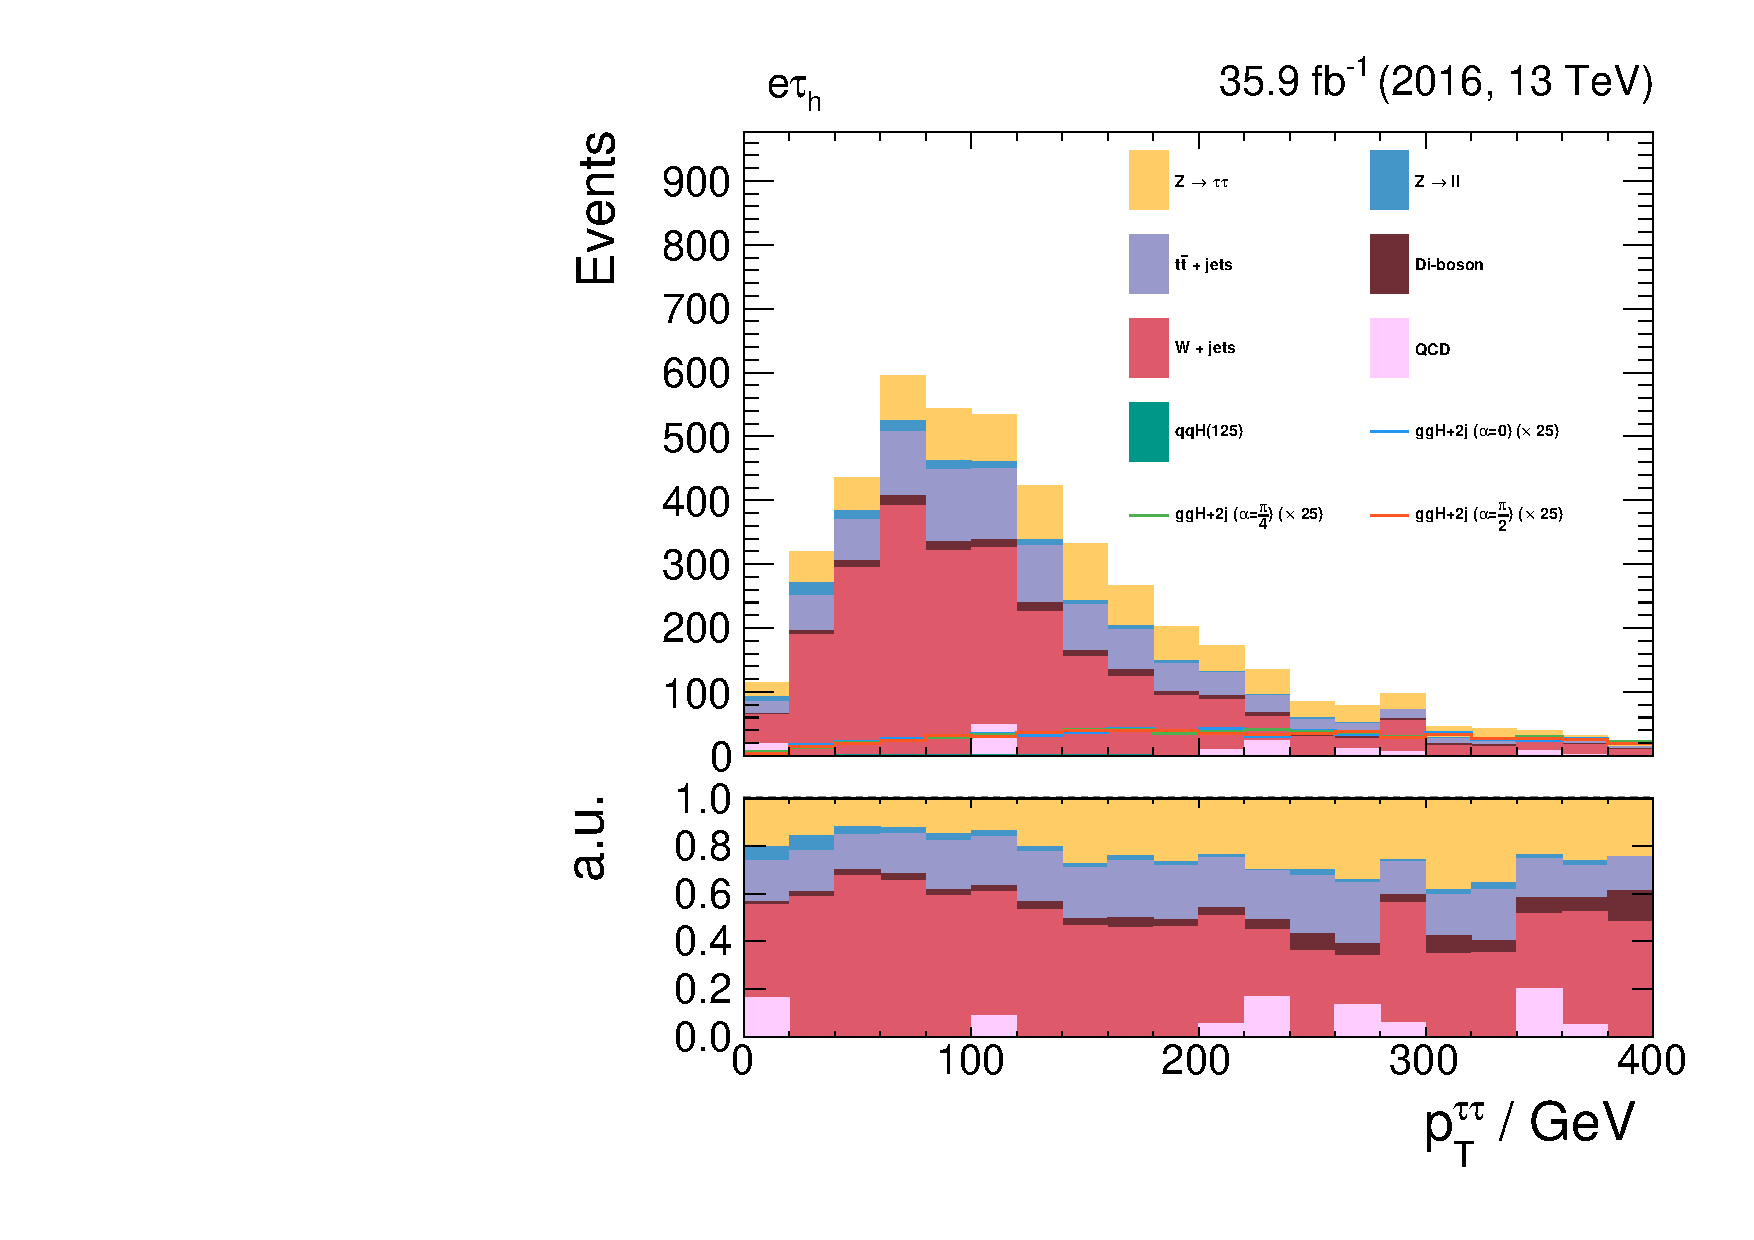
\includegraphics[width=\textwidth]{Figures/eventselection/Categorization/et/H_pt.pdf}
    \end{subfigure} \\ %
    \begin{subfigure}{.45\textwidth}
        \centering
        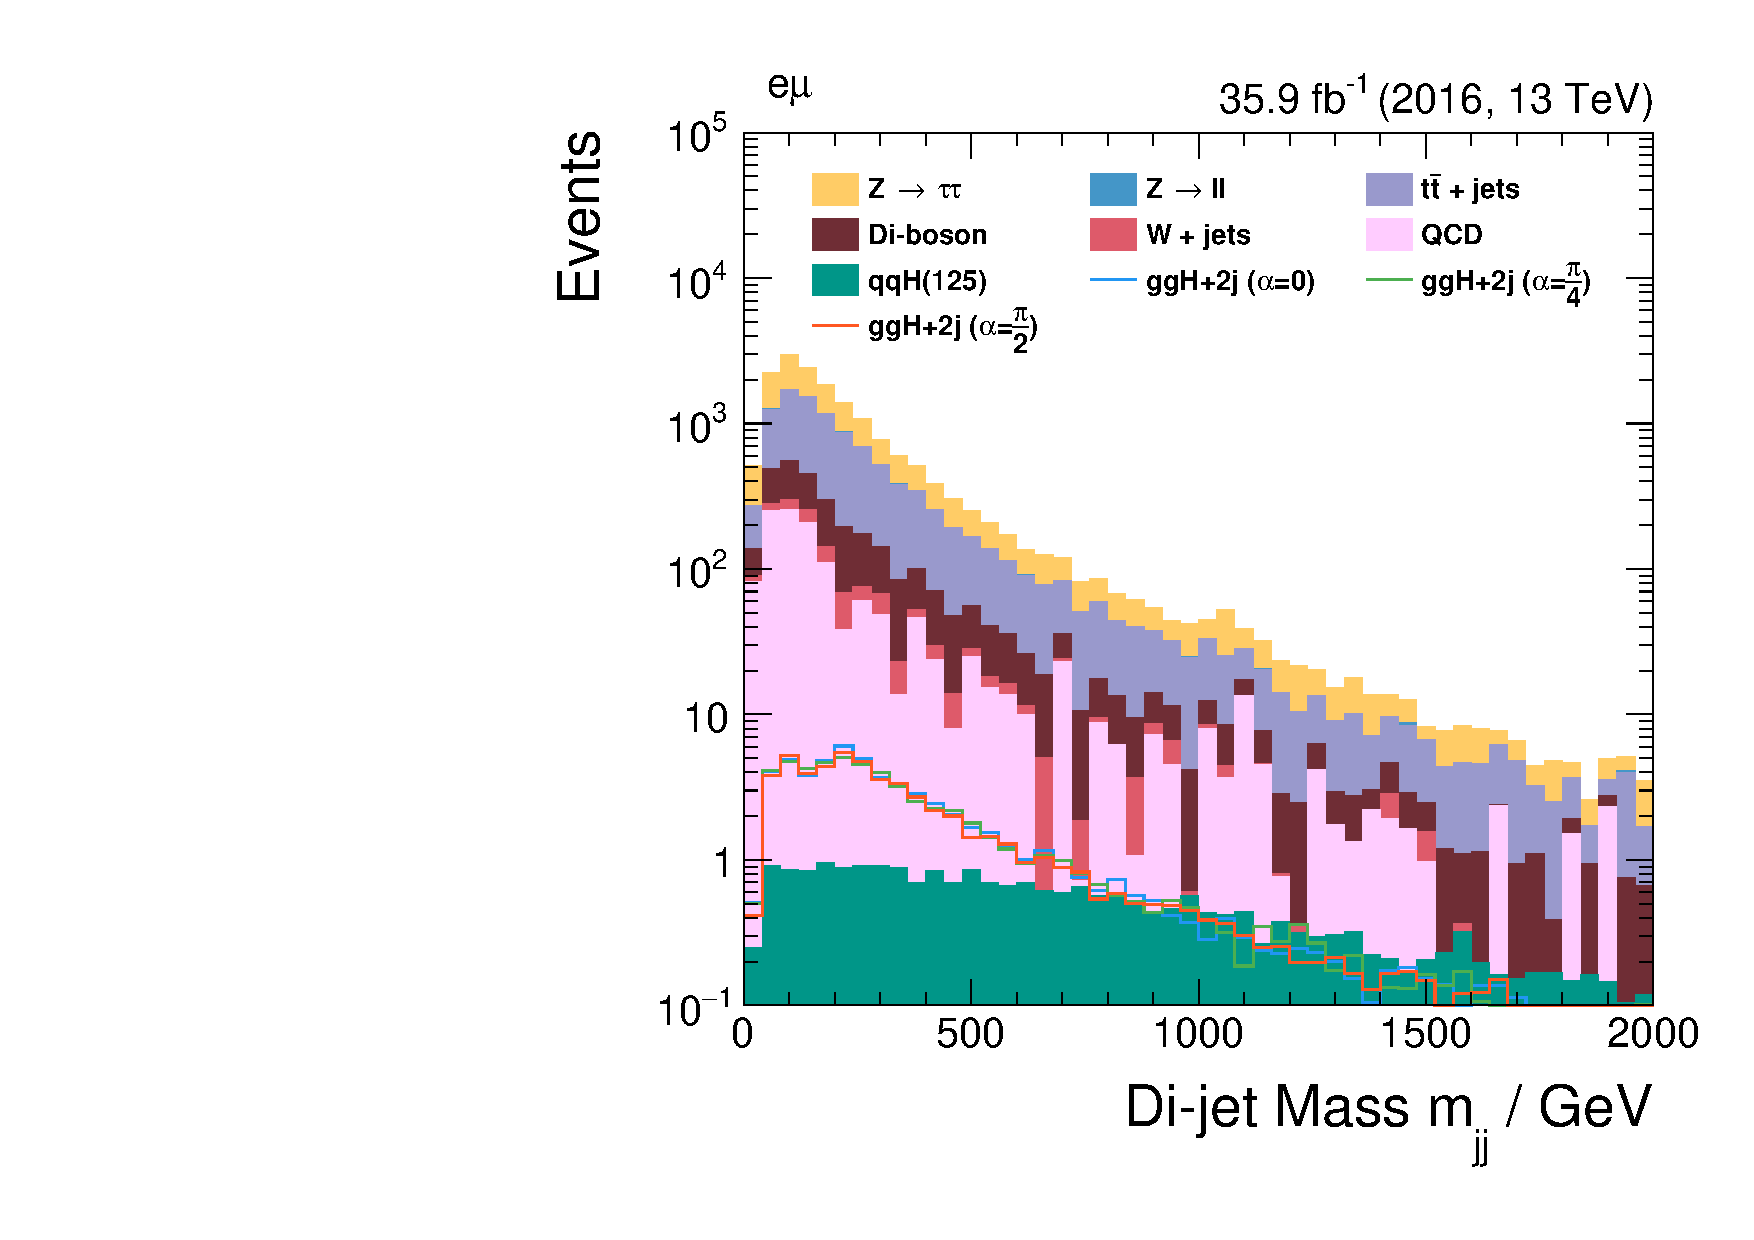
\includegraphics[width=\textwidth]{Figures/eventselection/Categorization/em/mjj.pdf}
    \end{subfigure}%
    \begin{subfigure}{.49\textwidth}
        \centering
        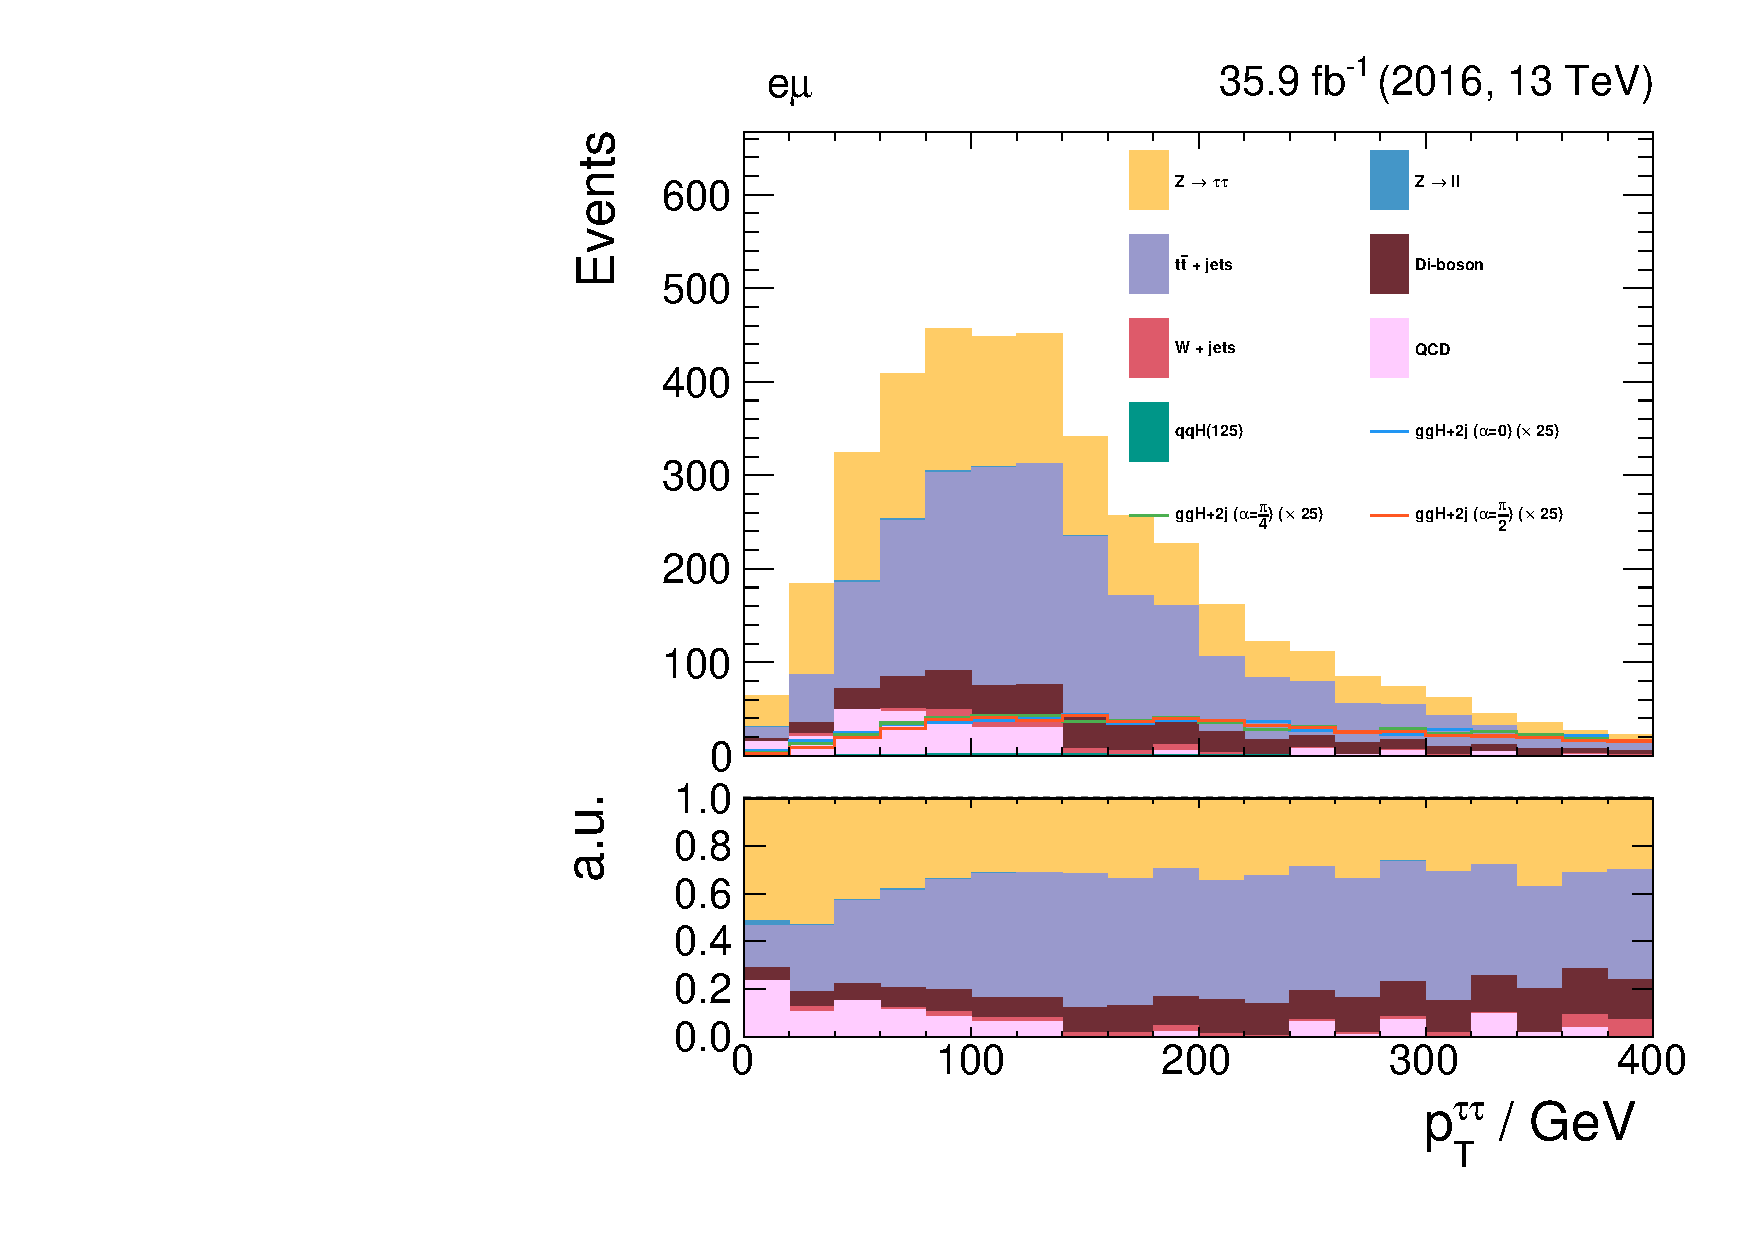
\includegraphics[width=\textwidth]{Figures/eventselection/Categorization/em/H_pt.pdf}
    \end{subfigure} %    
    \caption{Distributions of the invariant dijet mass $m_{jj}$ (left) and the reconstructed Higgs transverse momentum \ptautau{} (middle) for the \mutau{} (upper row), \etau{} (middle row) and $e\mu$ (bottom row) channels are shown for events with 2 jets or more.}\label{Supplement:ES:categorization:tt_distributions}
\end{figure}%

\clearpage
\begin{figure}[h!]
    \centering
    \begin{subfigure}{.3\textwidth}
        \centering
        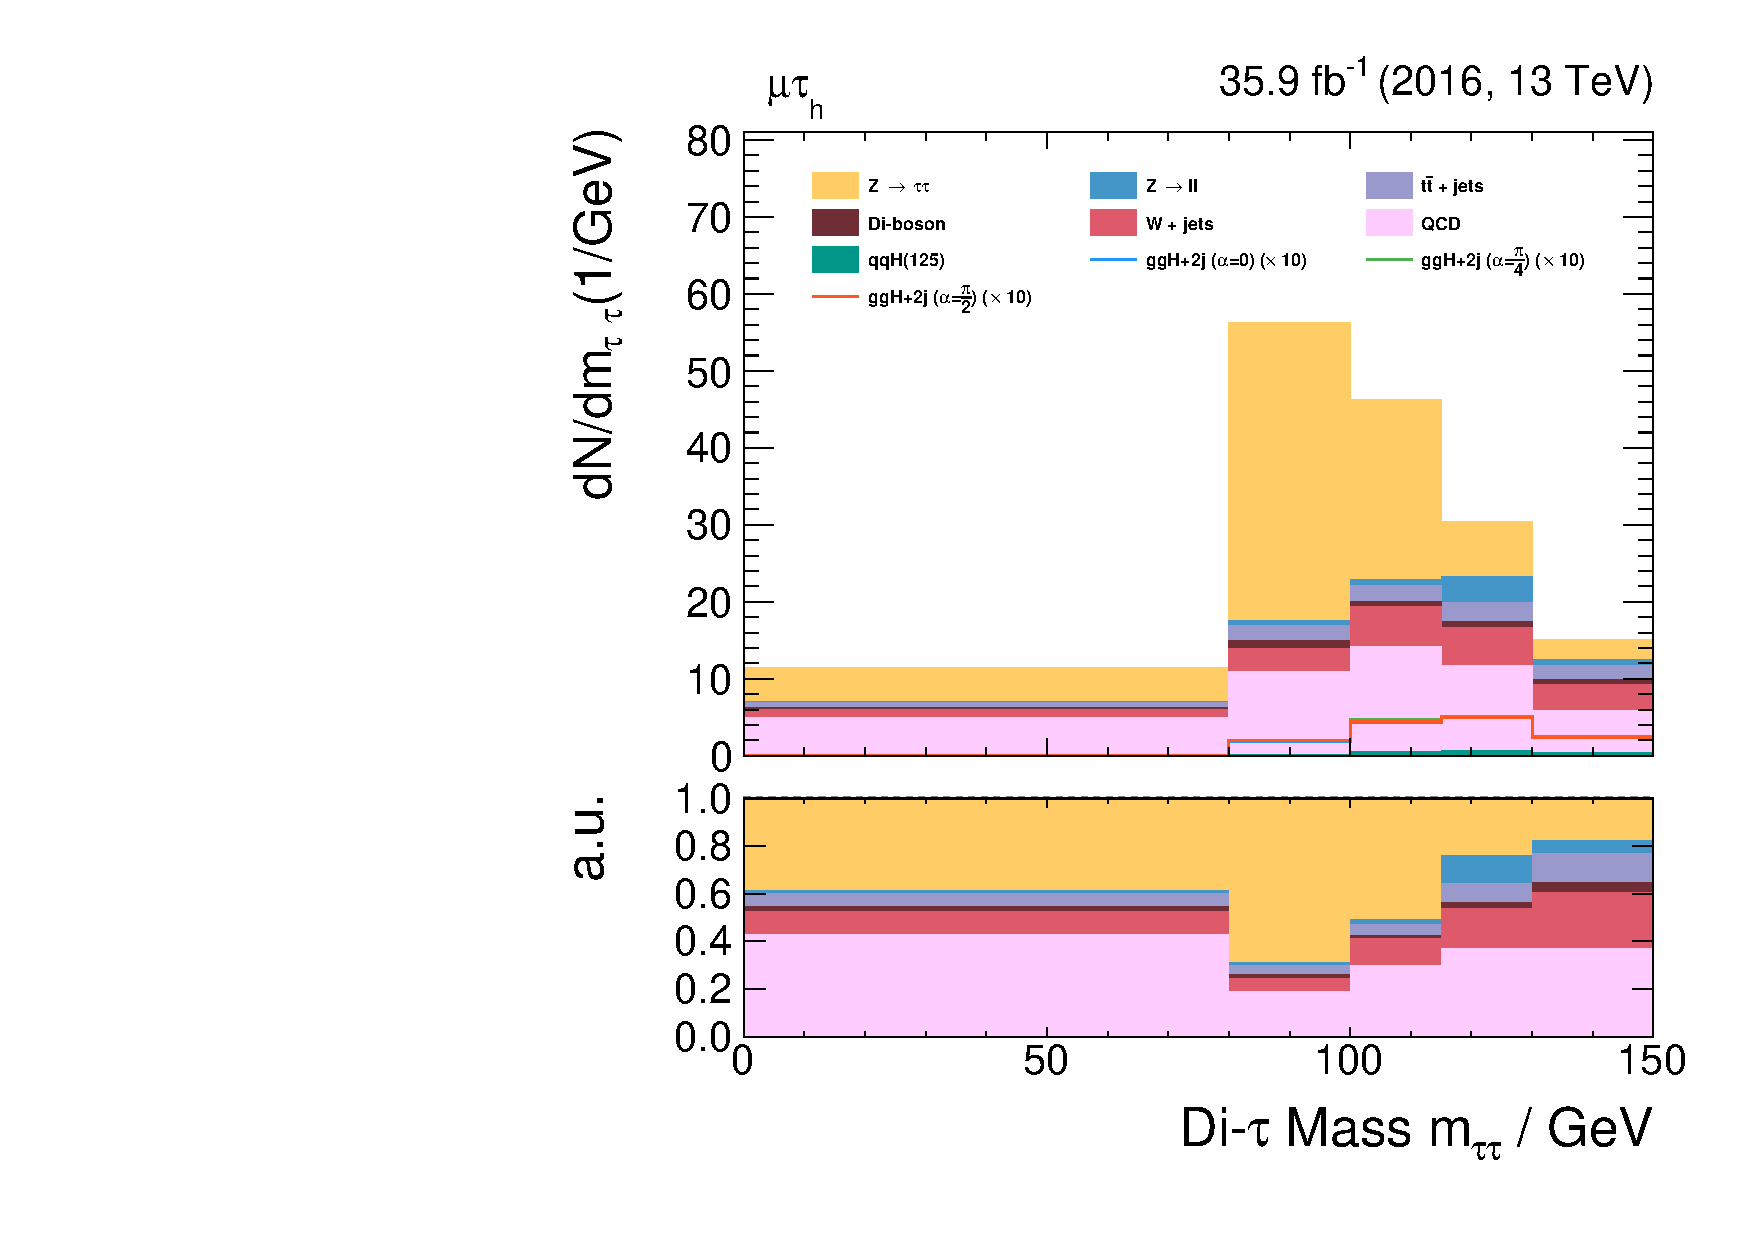
\includegraphics[width=\textwidth]{Figures/eventselection/mt/dijet2D_lowboost/m_sv.pdf}
    \end{subfigure}%
    \begin{subfigure}{.3\textwidth}
        \centering
        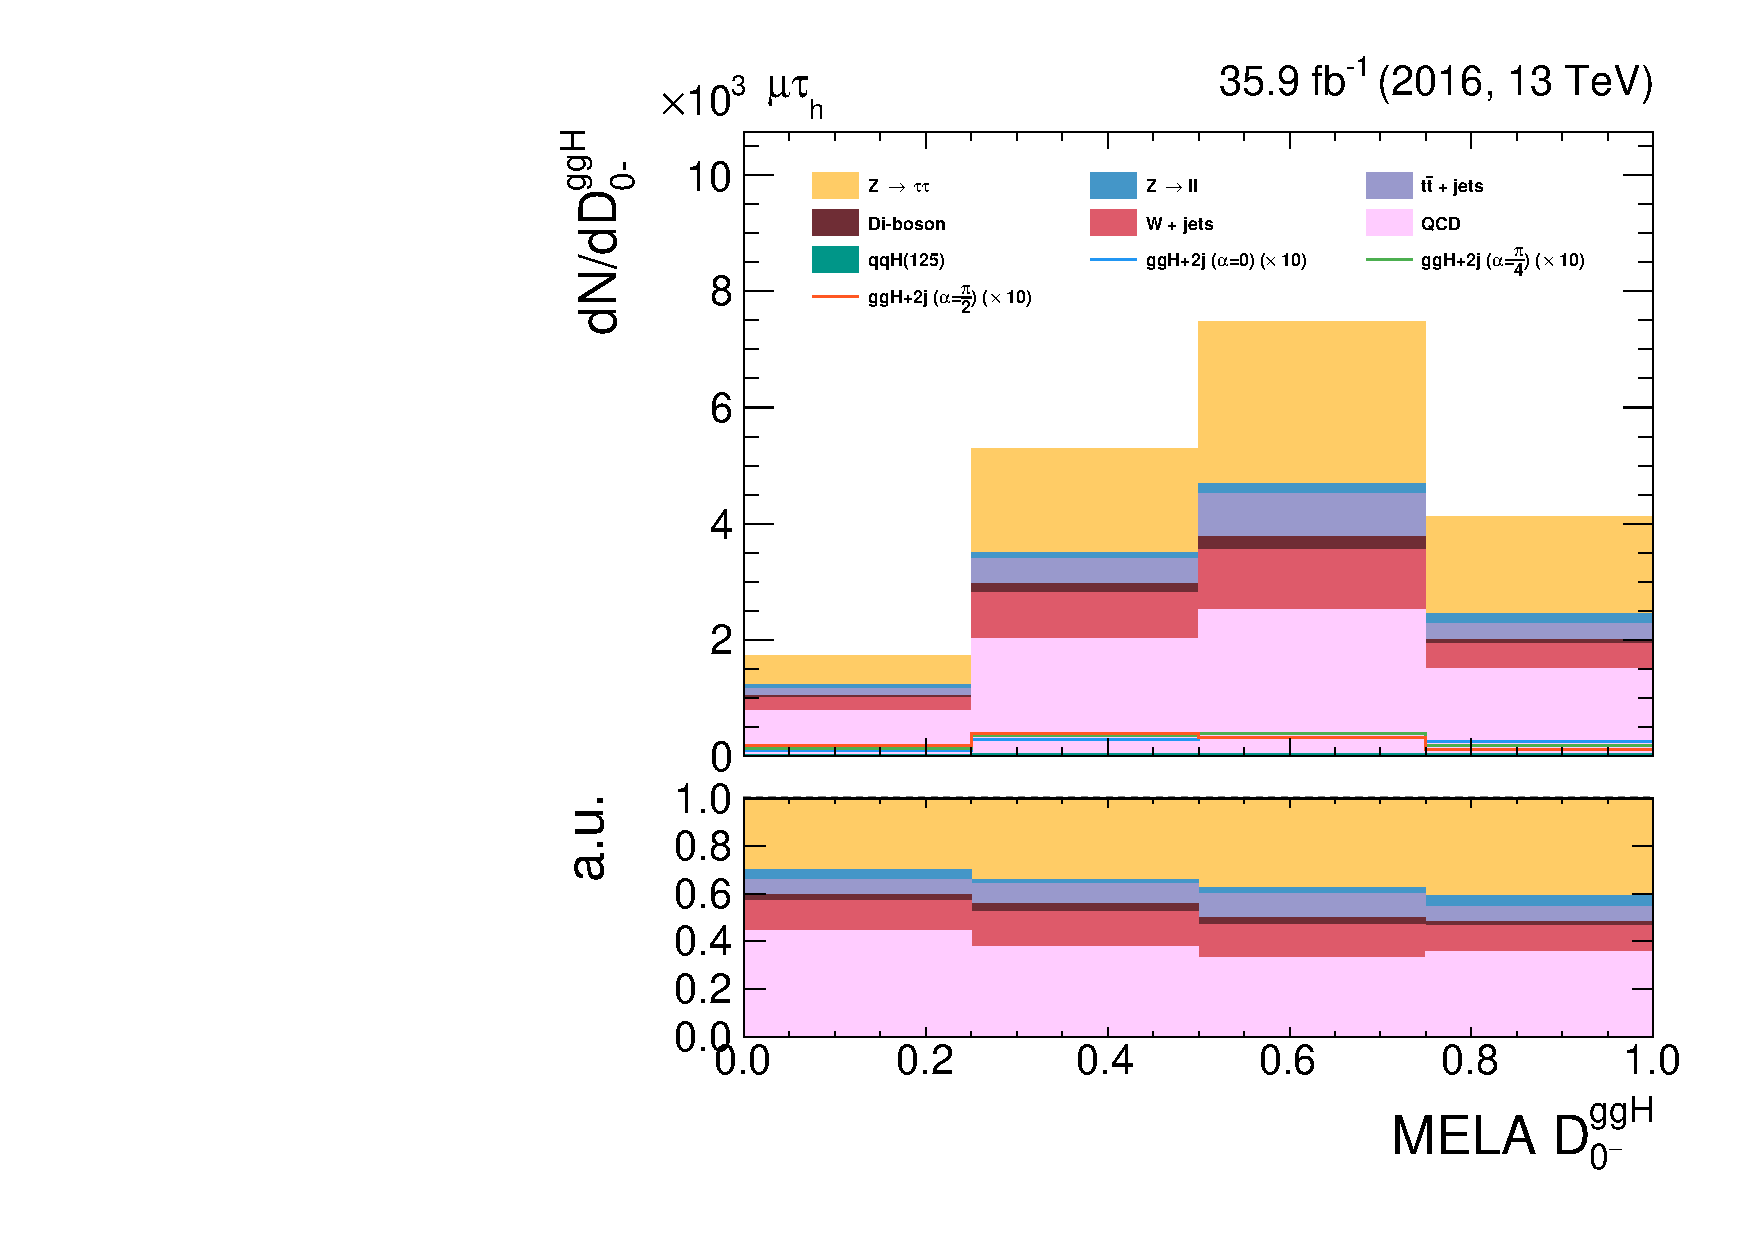
\includegraphics[width=\textwidth]{Figures/eventselection/mt/dijet2D_lowboost/melaDiscriminatorD0MinusGGH.pdf}
    \end{subfigure}%
    \begin{subfigure}{.3\textwidth}
        \centering
        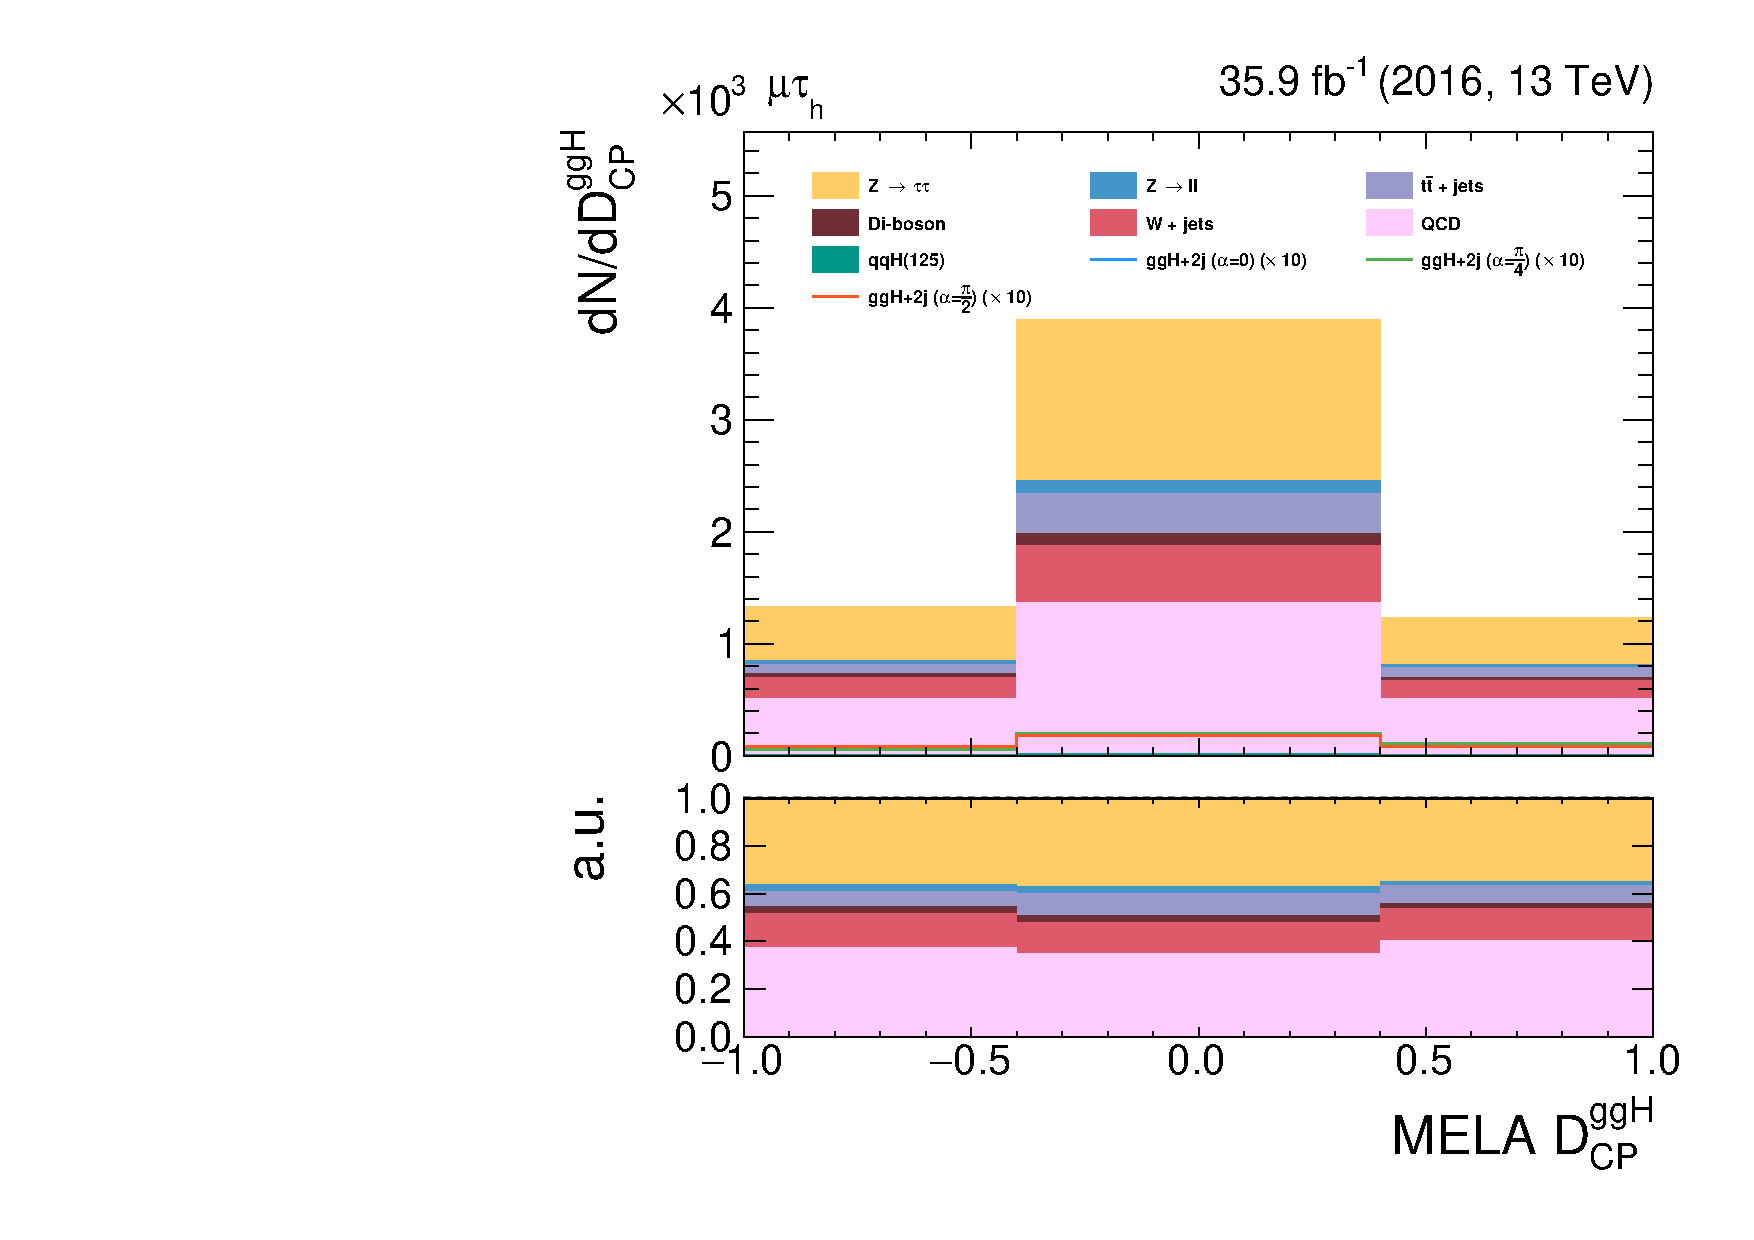
\includegraphics[width=\textwidth]{Figures/eventselection/mt/dijet2D_lowboost/melaDiscriminatorDCPGGH.pdf}
    \end{subfigure} \\ % 
    \begin{subfigure}{.3\textwidth}
        \centering
        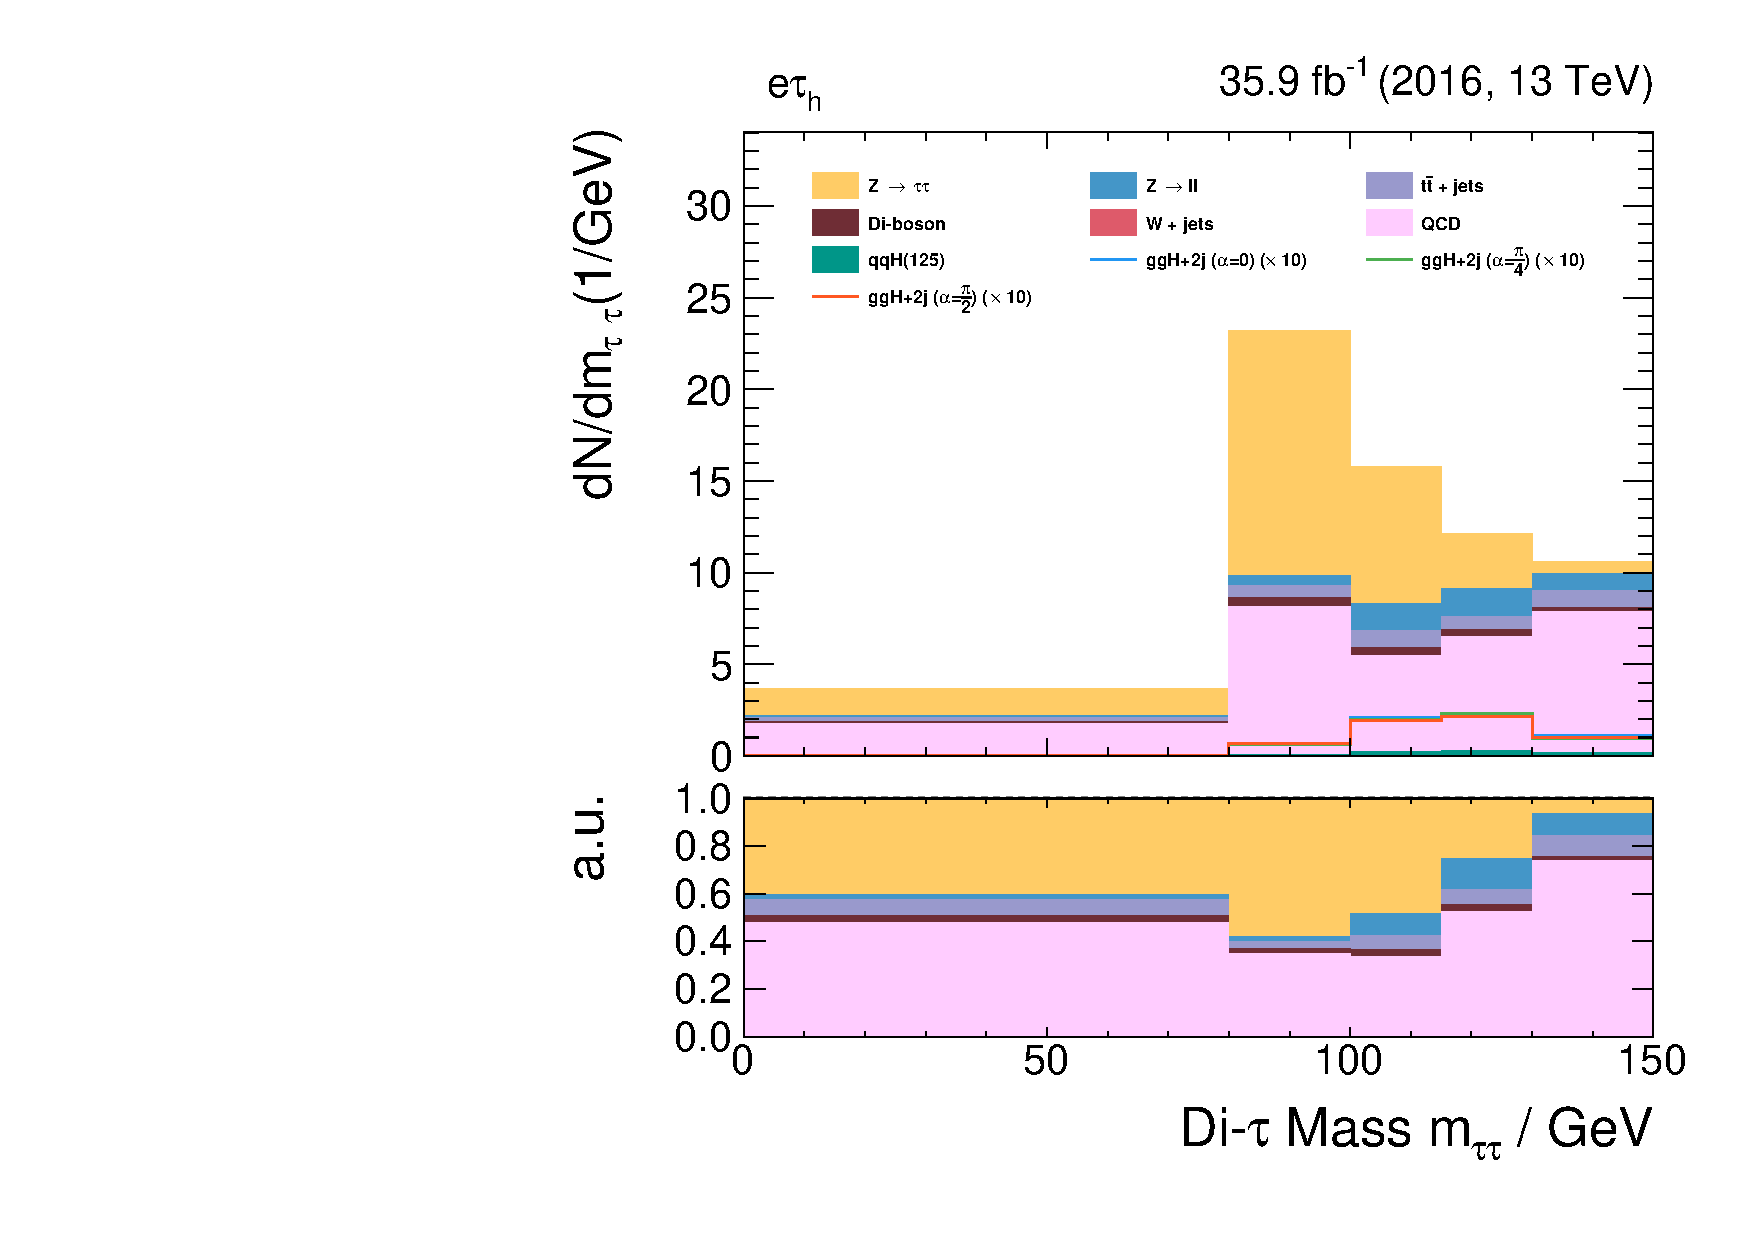
\includegraphics[width=\textwidth]{Figures/eventselection/et/dijet2D_lowboost/m_sv.pdf}
    \end{subfigure}%
    \begin{subfigure}{.3\textwidth}
        \centering
        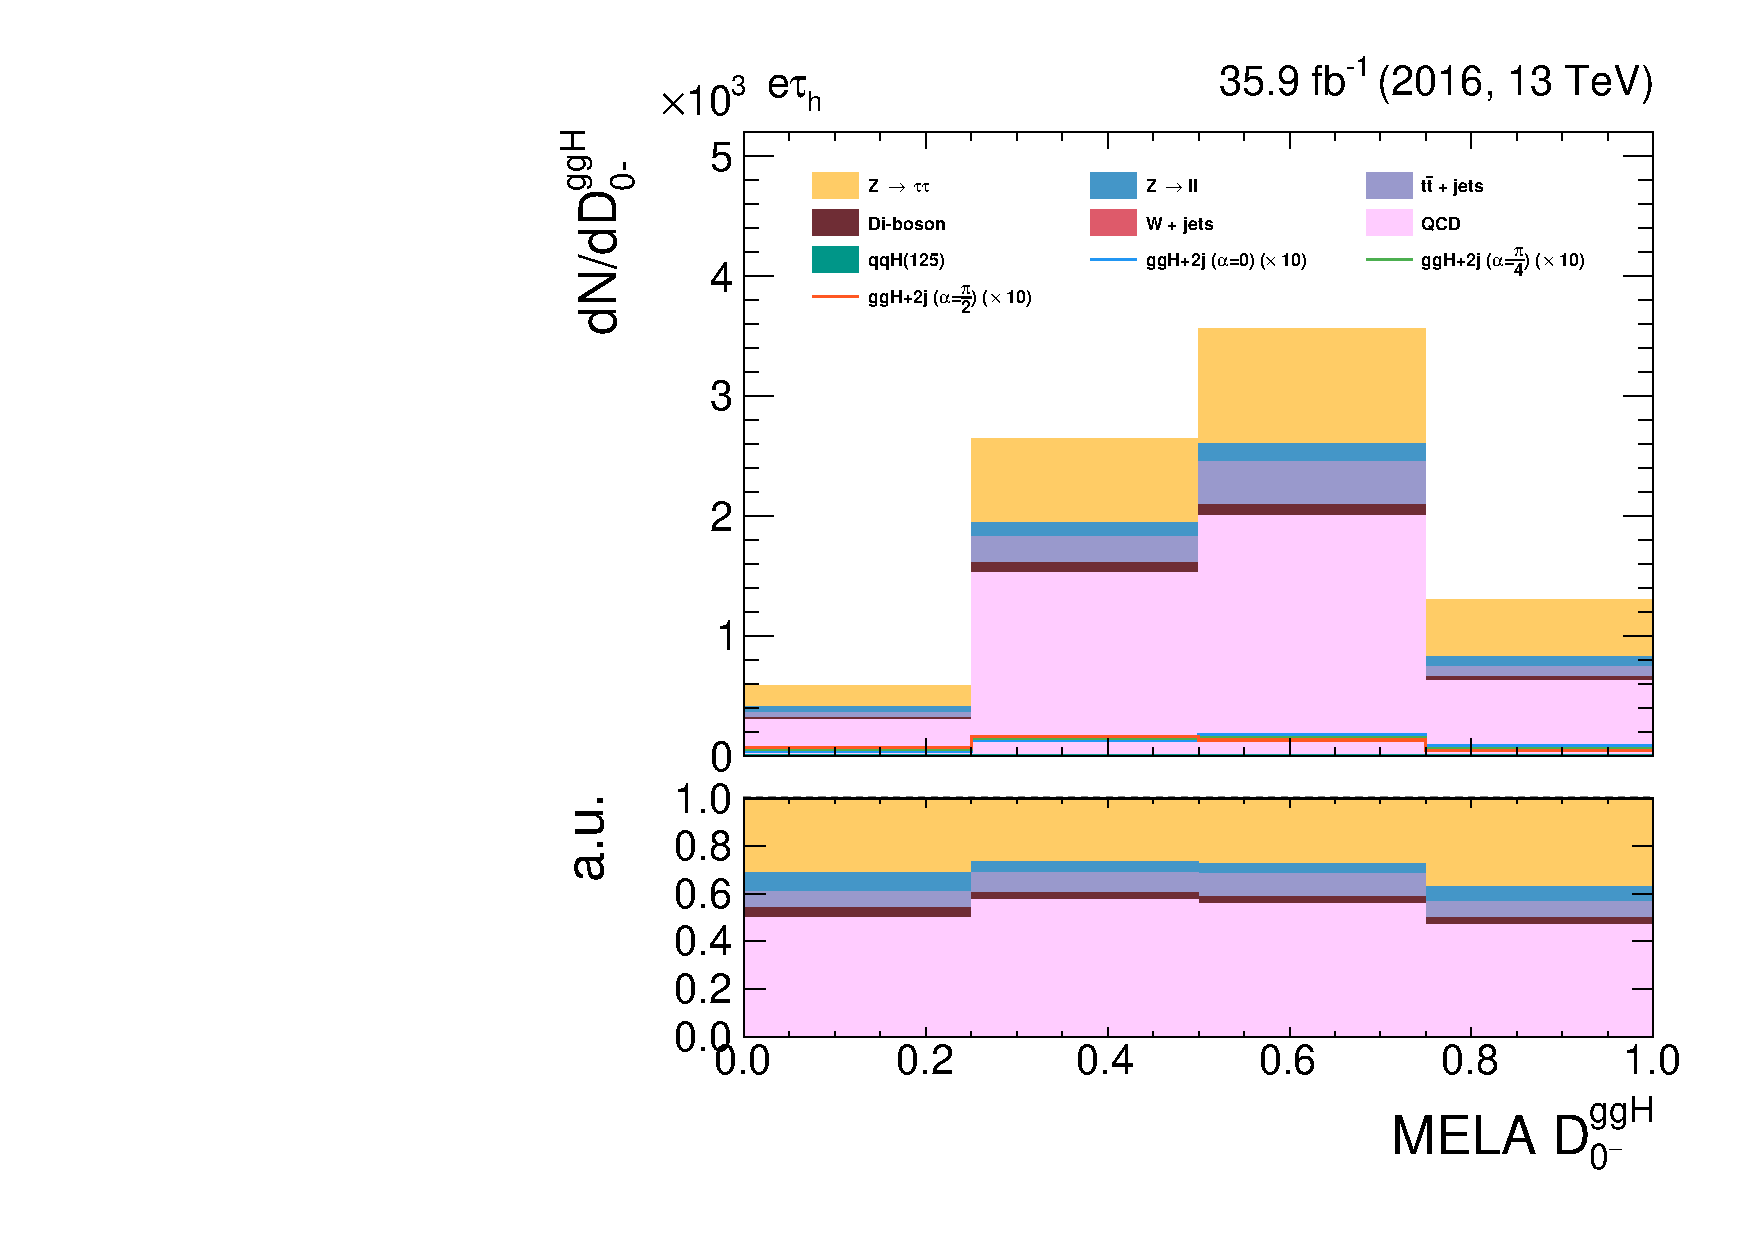
\includegraphics[width=\textwidth]{Figures/eventselection/et/dijet2D_lowboost/melaDiscriminatorD0MinusGGH.pdf}
    \end{subfigure}%
    \begin{subfigure}{.3\textwidth}
        \centering
        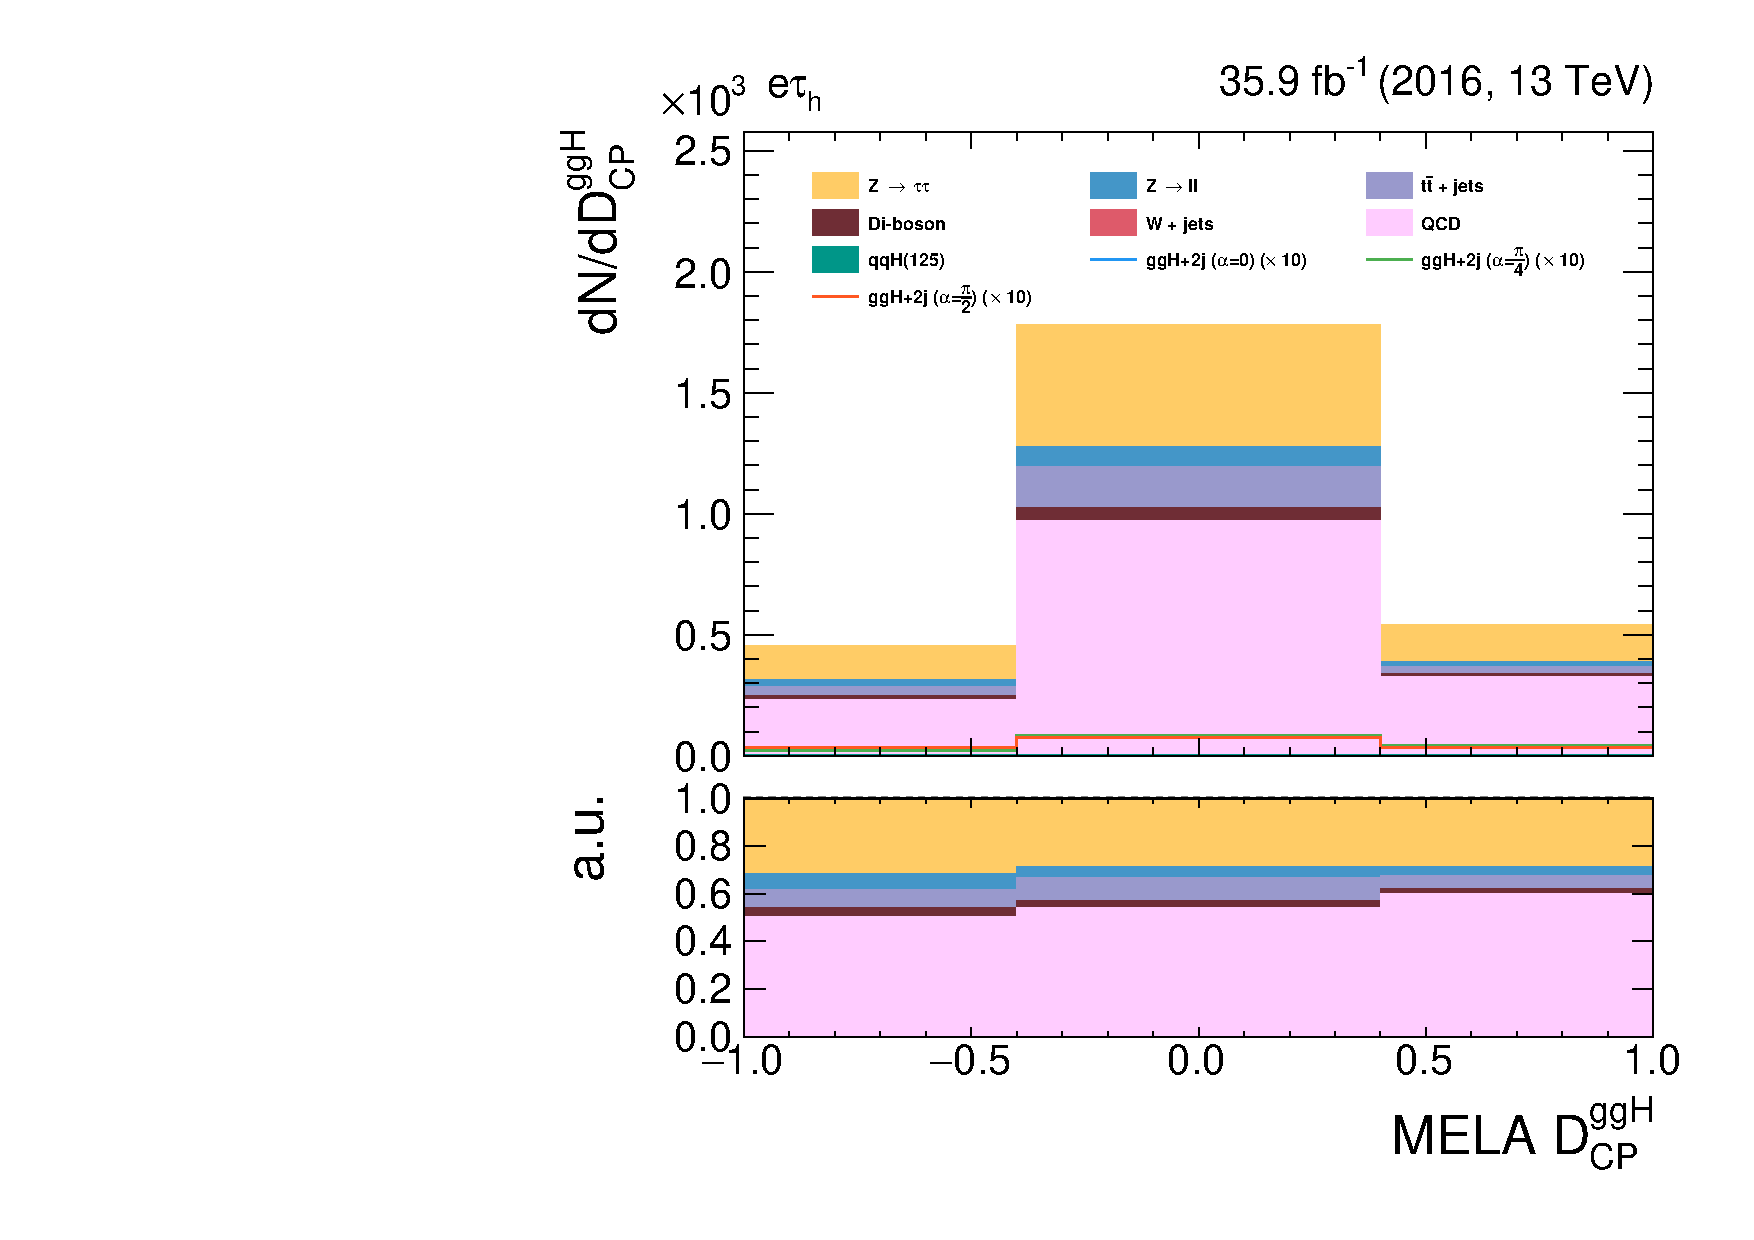
\includegraphics[width=\textwidth]{Figures/eventselection/et/dijet2D_lowboost/melaDiscriminatorDCPGGH.pdf}
    \end{subfigure} \\ % 
    \begin{subfigure}{.3\textwidth}
        \centering
        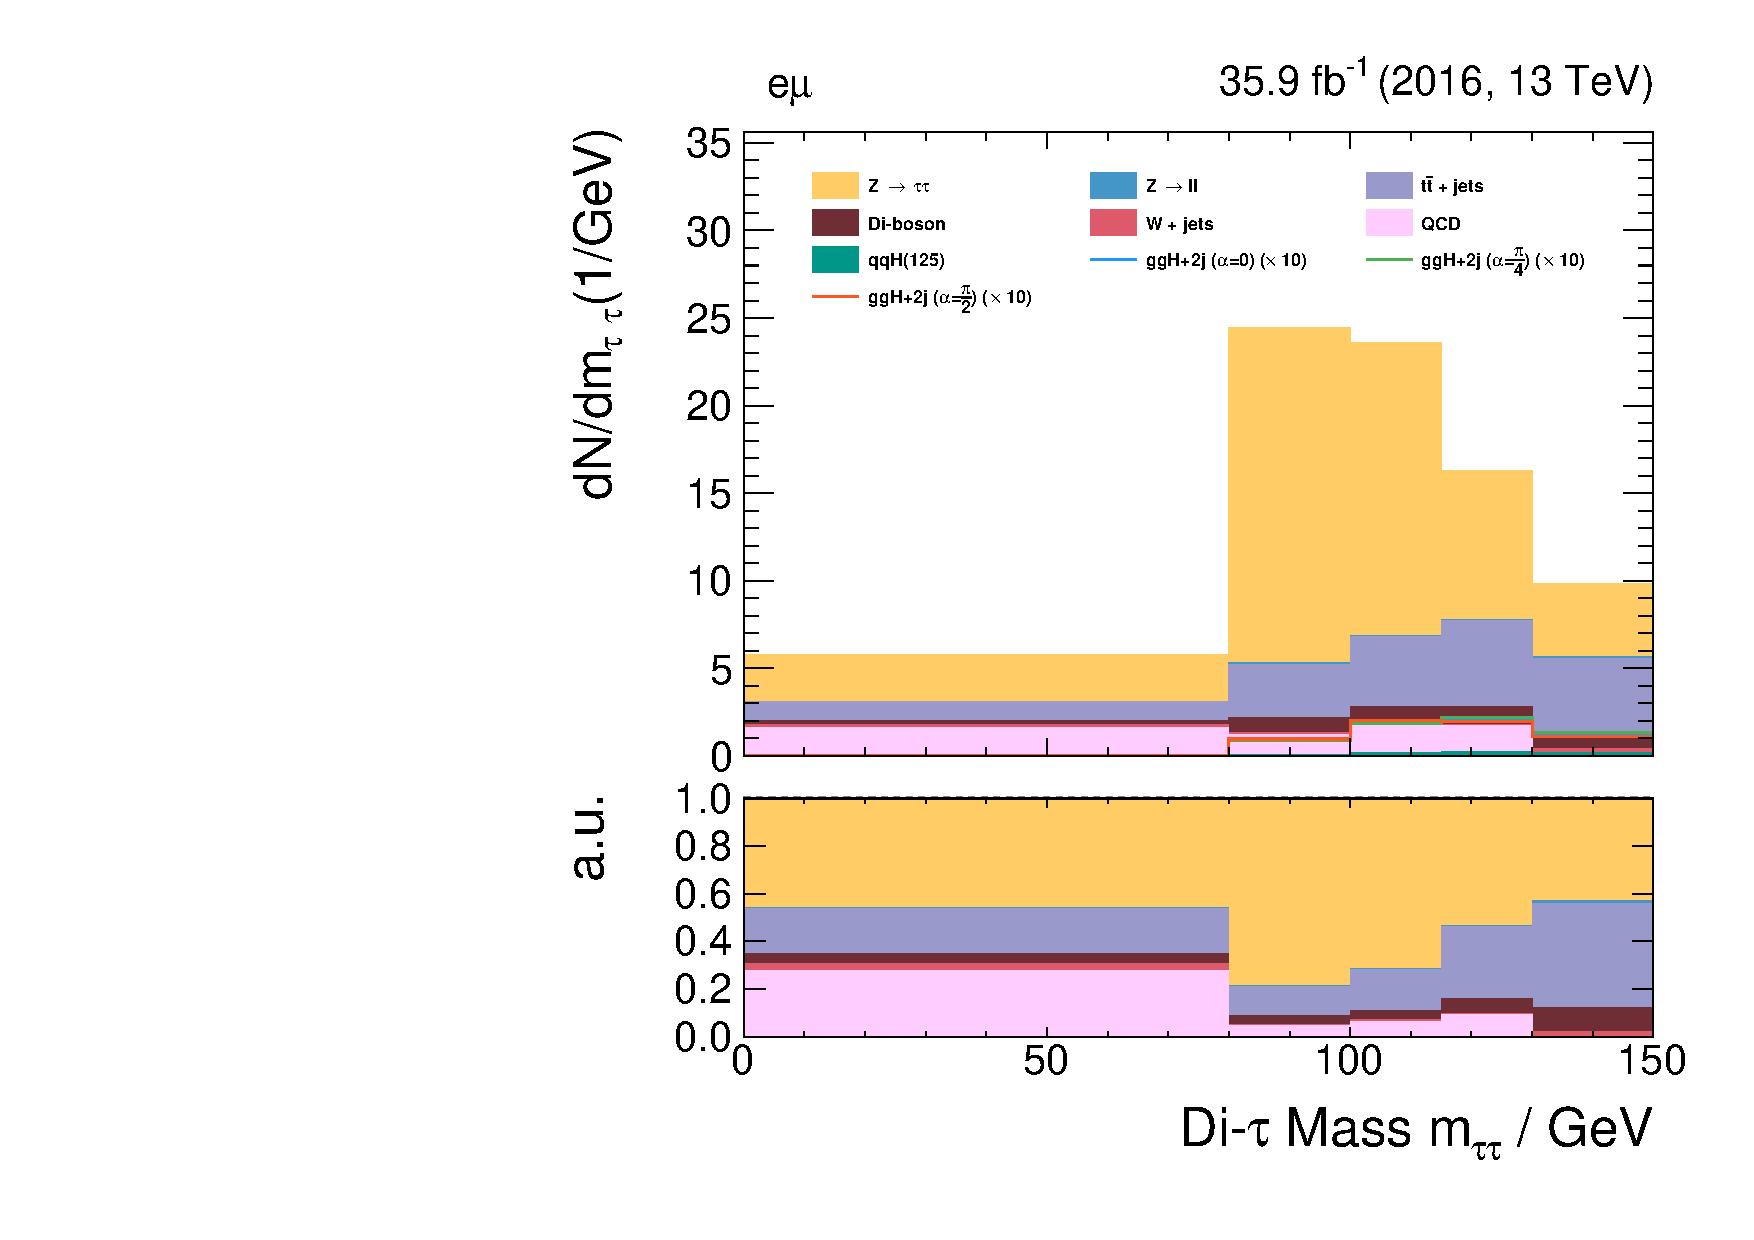
\includegraphics[width=\textwidth]{Figures/eventselection/em/dijet2D_lowboost/m_sv.pdf}
    \end{subfigure}%
    \begin{subfigure}{.3\textwidth}
        \centering
        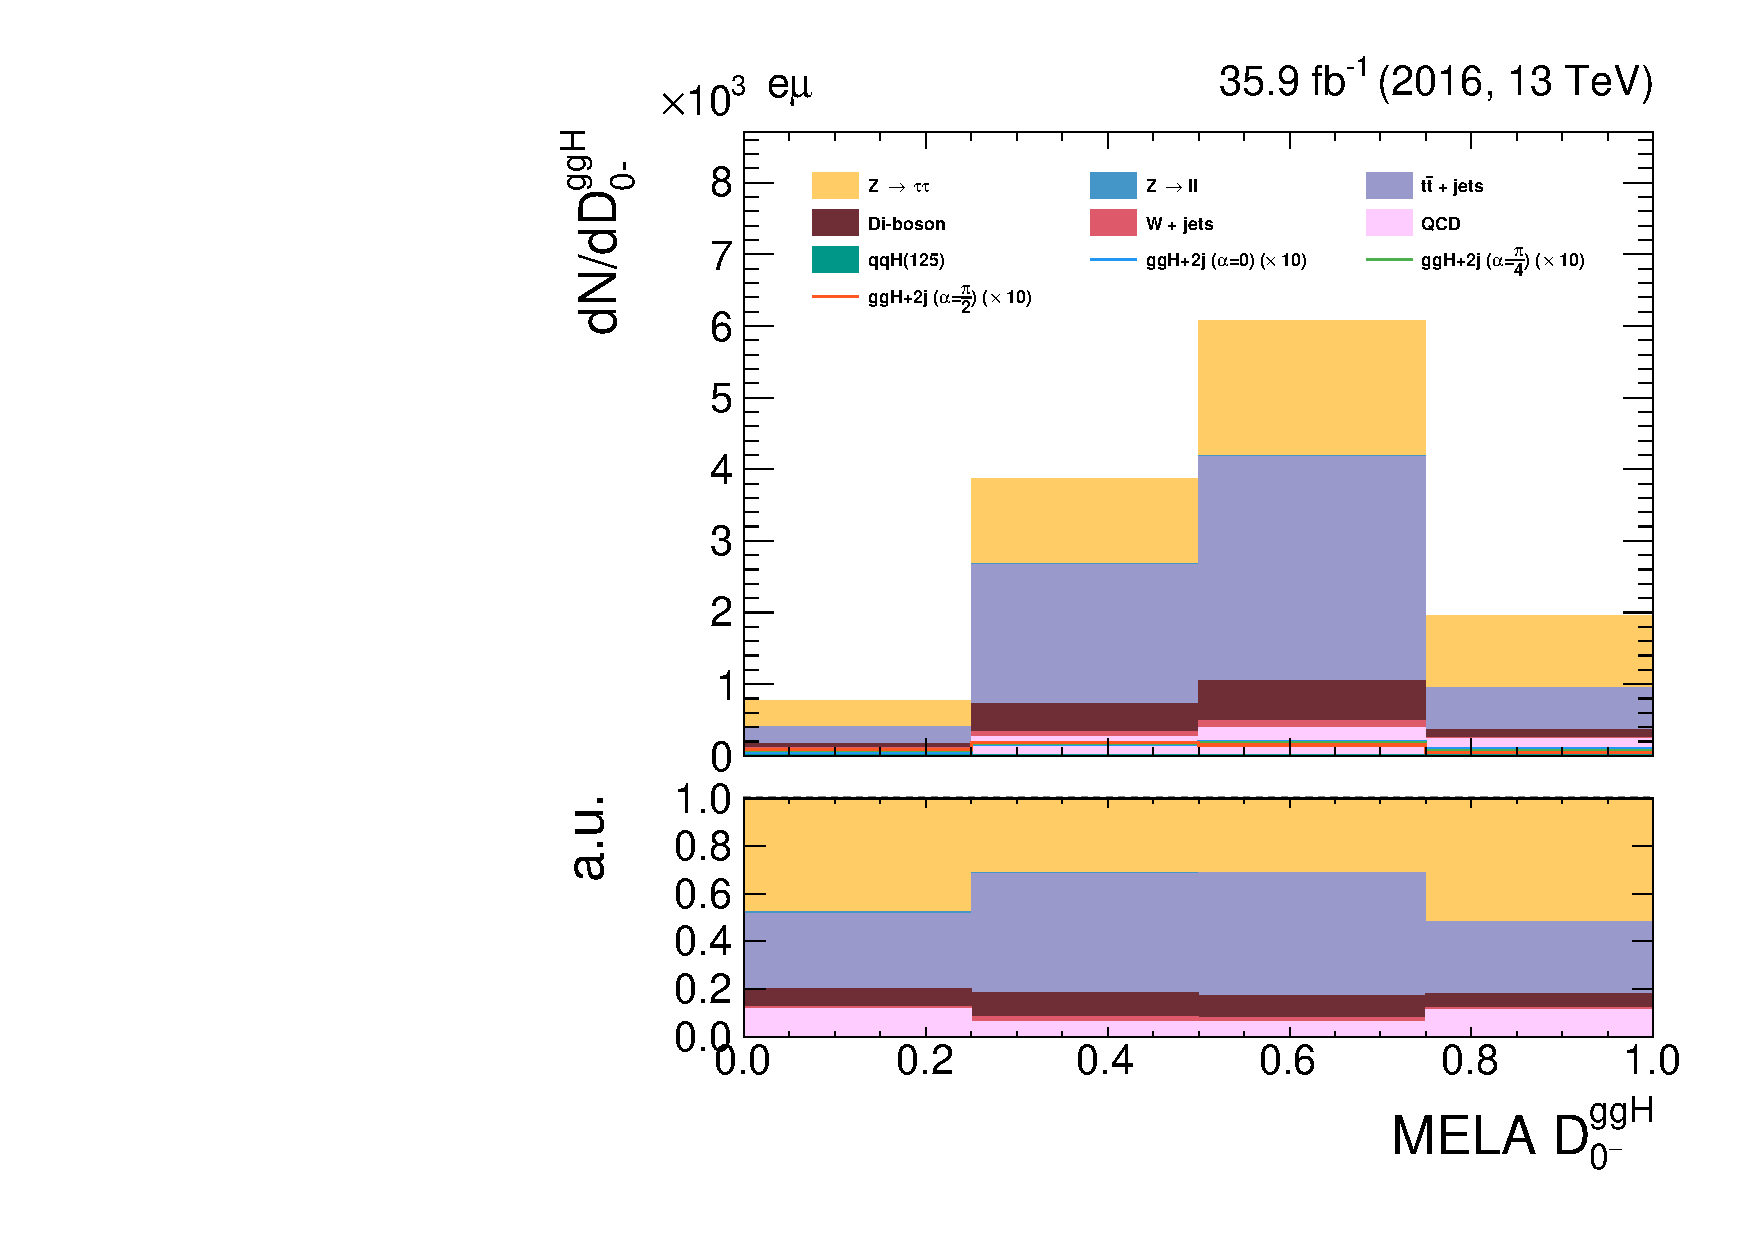
\includegraphics[width=\textwidth]{Figures/eventselection/em/dijet2D_lowboost/melaDiscriminatorD0MinusGGH.pdf}
    \end{subfigure}%
    \begin{subfigure}{.3\textwidth}
        \centering
        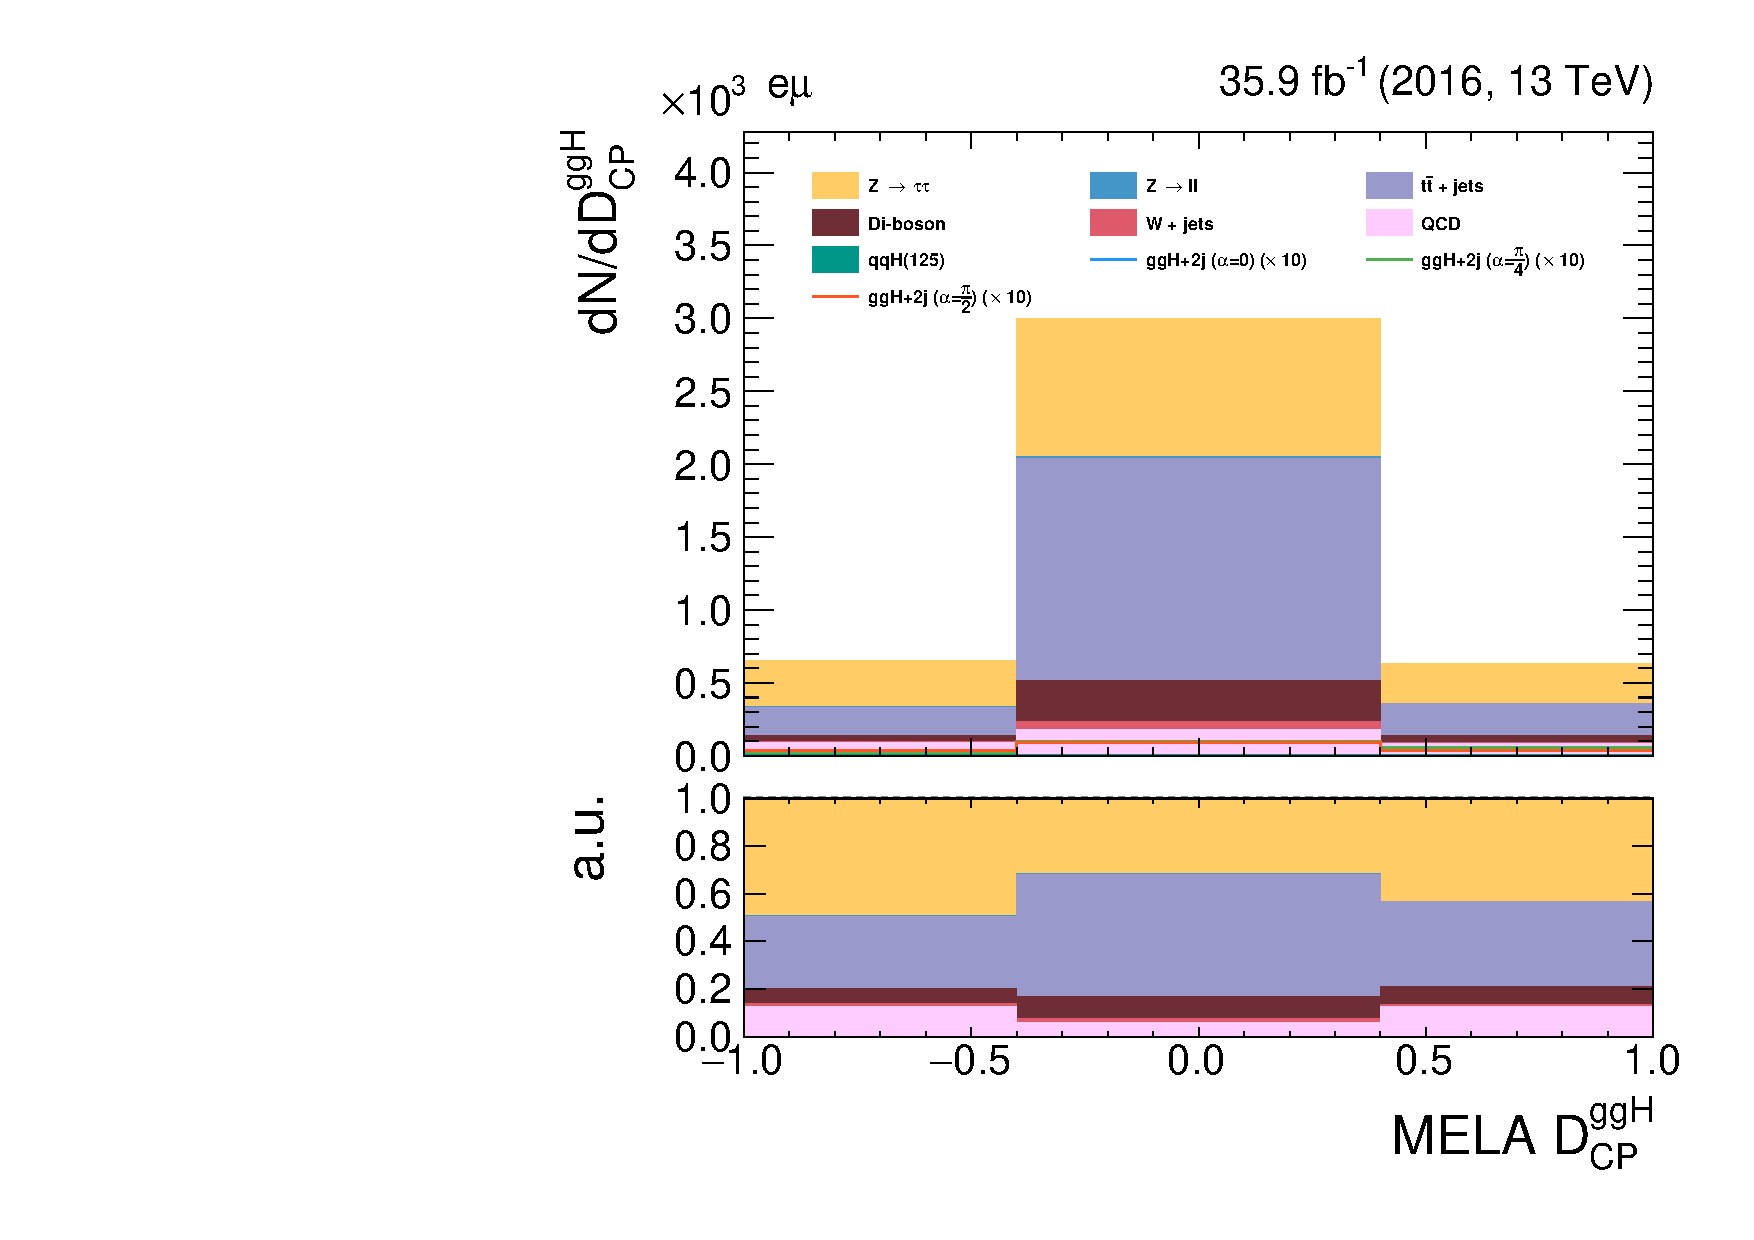
\includegraphics[width=\textwidth]{Figures/eventselection/em/dijet2D_lowboost/melaDiscriminatorDCPGGH.pdf}
    \end{subfigure}%         
    \caption{Background and ggH signal distributions for three scalar, maxmix and pseudoscalar CP scenarios of the observables in the 2-jet lowboost category for the \mutau{} (upper row), \etau (middle row) and $e\mu$ (bottom row) channels. 
    All histograms are normalized by the bin width and the ggH signal scaled by a factor 10.}\label{Supplement:ES:controlplots:2jet_lowboost}  
\end{figure}%
\clearpage
